\documentclass[a4paper, 10pt, ]{article}

\usepackage[slovak]{babel}





\usepackage[utf8]{inputenc}
\usepackage[T1]{fontenc}

\usepackage[left=4cm,
			right=4cm,
            % left=2.5cm,
			% right=5.5cm,
			top=2.1cm,
			bottom=2.6cm,
			footskip=7.5mm,
			% twoside,
			marginparwidth=3.0cm,
			%showframe,
			]{geometry}

\usepackage{graphicx}
\usepackage[dvipsnames]{xcolor}
% https://en.wikibooks.org/wiki/LaTeX/Colors


% ------------------------------

\usepackage{lmodern}

\usepackage[tt={oldstyle=false,proportional=true,monowidth}]{cfr-lm}

% ------------------------------

\usepackage{amsmath}
\usepackage{amssymb}
\usepackage{amsthm}

\usepackage{booktabs}
\usepackage{multirow}
\usepackage{array}
\usepackage{dcolumn}


\usepackage[singlelinecheck=true]{subfig}


% ------------------------------


\def\naT{\mathsf{T}}

\hyphenpenalty=6000
\tolerance=1000




% ------------------------------


\makeatletter

	\def\@seccntformat#1{\protect\makebox[0pt][r]{\csname the#1\endcsname\hspace{4mm}}}

	\def\cleardoublepage{\clearpage\if@twoside \ifodd\c@page\else
	\hbox{}
	\vspace*{\fill}
	\begin{center}
	\phantom{}
	\end{center}
	\vspace{\fill}
	\thispagestyle{empty}
	\newpage
	\if@twocolumn\hbox{}\newpage\fi\fi\fi}

	\newcommand\figcaption{\def\@captype{figure}\caption}
	\newcommand\tabcaption{\def\@captype{table}\caption}

\makeatother


% ------------------------------




\usepackage{fancyhdr}
\fancypagestyle{plain}{%
\fancyhf{} % clear all header and footer fields
\fancyfoot[C]{\sffamily {\bfseries \thepage}\ | {\scriptsize\oznacenieCasti}}
\renewcommand{\headrulewidth}{0pt}
\renewcommand{\footrulewidth}{0pt}}
\pagestyle{plain}


% ------------------------------


\usepackage{titlesec}
\titleformat{\paragraph}[hang]{\sffamily  \bfseries}{}{0pt}{}
\titlespacing*{\paragraph}{0mm}{3mm}{1mm}
\titlespacing*{\subparagraph}{0mm}{3mm}{1mm}

\titleformat*{\section}{\sffamily\Large\bfseries}
\titleformat*{\subsection}{\sffamily\large\bfseries}
\titleformat*{\subsubsection}{\sffamily\normalsize\bfseries}






% ------------------------------

\PassOptionsToPackage{hyphens}{url}
\usepackage[pdfauthor={},
			pdftitle={},
			pdfsubject={},
			pdfkeywords={},
			% hidelinks,
			colorlinks=false,
			breaklinks,
			]{hyperref}


% ------------------------------


\graphicspath{%
{../fig_standalone/}%
{../../PY/fig/}%
{../../PY/jupynotex/fig/}%
{../../ML/fig/}%
{./fig/}%
}



% ------------------------------

\usepackage{enumitem}

\usepackage{lettrine}

% ------------------------------


\usepackage{microtype}


% ------------------------------

\usepackage[titles]{tocloft}

\setlength{\cftsecindent}{-12mm}
\setlength{\cftsecnumwidth}{12mm}
\renewcommand{\cftsecpresnum}{\hfill}
\renewcommand{\cftsecaftersnum}{\hspace{4mm}}

\setlength{\cftsubsecindent}{-12mm}
\setlength{\cftsubsecnumwidth}{16mm} % 12 + 4
\renewcommand{\cftsubsecpresnum}{\hfill}
\renewcommand{\cftsubsecaftersnum}{\hspace{8mm}} % 4 + 4 mm

\setlength{\cftsubsubsecindent}{-12mm}
\setlength{\cftsubsubsecnumwidth}{20mm} % 12 + 4 + 4
\renewcommand{\cftsubsubsecpresnum}{\hfill}
\renewcommand{\cftsubsubsecaftersnum}{\hspace{12mm}} % 4 + 4 + 4 mm

\renewcommand{\cftsecpagefont}{\lstyle \bfseries}
\renewcommand{\cftsubsecpagefont}{\lstyle}
\renewcommand{\cftsubsubsecpagefont}{\lstyle}



\setlength{\cftparaindent}{-16mm}
\setlength{\cftparanumwidth}{28mm} % 16 + 4 + 4 + 4
\renewcommand{\cftparapresnum}{\hfill}
\renewcommand{\cftparaaftersnum}{\hspace{16mm}} % 4 + 4 + 4 + 4 mm








% ------------------------------

\usepackage{listings}



\renewcommand{\lstlistingname}{Výpis kódu}
\renewcommand{\lstlistlistingname}{Výpisy kódu}




%New colors defined below
\definecolor{codegreen}{rgb}{0,0.6,0}
\definecolor{codegray}{rgb}{0.5,0.5,0.5}
\definecolor{codepurple}{rgb}{0.58,0,0.82}
\definecolor{backcolour}{rgb}{0.95,0.95,0.95}

%Code listing style named "mystyle"
\lstdefinestyle{mystyle}{
  backgroundcolor=\color{backcolour},
  commentstyle=\fontfamily{lmtt}\fontsize{8.5pt}{8.75pt}\selectfont\color{codegreen},
  keywordstyle=\fontfamily{lmtt}\fontsize{8.5pt}{8.75pt}\selectfont\bfseries\color{Blue},
  stringstyle=\fontfamily{lmtt}\fontsize{8.5pt}{8.75pt}\selectfont\color{codepurple},
  basicstyle=\fontfamily{lmtt}\fontsize{8.5pt}{8.75pt}\selectfont,
  breakatwhitespace=false,
  breaklines=true,
  captionpos=t,
  keepspaces=true,
  numbers=left,
  numbersep=4mm,
  numberstyle=\fontfamily{lmtt}\fontsize{8.5pt}{8.75pt}\selectfont\color{lightgray},
  showspaces=false,
  showstringspaces=false,
  showtabs=false,
  tabsize=2,
  % xleftmargin=10pt,
  framesep=10pt,
  language=Python,
  escapechar=|,
}


\lstset{
    inputencoding=utf8,
    extendedchars=true,
    literate=%
    {á}{{\'a}}1
    {č}{{\v{c}}}1
    {ď}{{\v{d}}}1
    {é}{{\'e}}1
    {ě}{{\v{e}}}1
    {í}{{\'i}}1
    {ň}{{\v{n}}}1
    {ó}{{\'o}}1
    {ř}{{\v{r}}}1
    {š}{{\v{s}}}1
    {ť}{{\v{t}}}1
    {ú}{{\'u}}1
    {ů}{{\r{u}}}1
    {ý}{{\'y}}1
    {ž}{{\v{z}}}1
    {Á}{{\'A}}1
    {Č}{{\v{C}}}1
    {Ď}{{\v{D}}}1
    {É}{{\'E}}1
    {Ě}{{\v{E}}}1
    {Í}{{\'I}}1
    {Ň}{{\v{N}}}1
    {Ó}{{\'O}}1
    {Ř}{{\v{R}}}1
    {Š}{{\v{S}}}1
    {Ť}{{\v{T}}}1
    {Ú}{{\'U}}1
    {Ů}{{\r{U}}}1
    {Ý}{{\'Y}}1
    {Ž}{{\v{Z}}}1
    {ô}{{\^{o}}}1
}


% ------------------------------


\usepackage{caption}

\DeclareCaptionFormat{odsadene}{\protect\makebox[0pt][r]{#1#2\hspace{4mm}}#3\par}
\DeclareCaptionLabelSeparator{lendvojbodka}{:}
% \DeclareCaptionFont{lightgray}{\color{lightgray}}
\DeclareCaptionFont{lightgray}{\fontfamily{lmtt}\fontsize{8.5pt}{8.75pt}\selectfont\color{lightgray}}

\captionsetup[lstlisting]{format=odsadene, labelsep=lendvojbodka, justification=raggedright, singlelinecheck=false, labelfont={sf, lightgray},}


% ------------------------------





% ------------------------------

\usepackage[backend=biber,
            style=numeric,
            sorting=none,
            ]{biblatex}
\DeclareSourcemap{
    \maps[datatype=bibtex]{
        \map{
        \step[fieldset=note, null]
        }
        \map{
        \step[fieldset=file, null]
        }        
        % \map{
        % \step[fieldset=url, null]        
        % }
        \map{
        \step[fieldset=eprint, null]
        }
    }
}


\addbibresource{E:/_CurrentContent/01_work_repo/bibLaTeXDB/bibLaTeXDB.bib} % nonpublic data





\def\oznacenieCasti{MRS07 - ZS2025}


\usepackage{longtable}




\begin{document}


\lstset{%
style=mystyle,
rangebeginprefix=\#\#\#\ cellB\ ,%
rangebeginsuffix=\ \#\#\#,%
rangeendprefix=\#\#\#\ cellE\ ,%
rangeendsuffix=\ \#\#\#,%
includerangemarker=false,
}





\fontsize{12pt}{22pt}\selectfont

\centerline{\textsf{Modelovanie a riadenie systémov} \hfill \textsf{\oznacenieCasti}}

\fontsize{18pt}{22pt}\selectfont





\begin{flushleft}
	\textbf{\textsf{Laplaceova transformácia,\\ prenosové funkcie, modelovanie systémov}}
\end{flushleft}





\normalsize

% \bigskip

{\hypersetup{hidelinks}

\tableofcontents

}

\bigskip

\vspace{18pt}



\noindent
\lettrine[lines=3, nindent=0pt]{L}{aplaceova} transformácia umožňuje efektívne pracovať s lineárnymi dynamickými systémami. Transformuje a tým zjednodušuje operácie súvisiace s hľadaním riešenia lineárnych diferenciálnych rovníc (LDR). Predovšetkým zjednodušuje prácu s konvolučnou rovnicou (konvolučným integrálom) (pozri časť~\ref{predchcasttato}).

K využitiu Laplaceovej transformácie pri riešení diferenciálnych rovníc patrí aj pojem \emph{prenosová funkcia}. Ak hovoríme o prenosových funkciách, hovoríme o nástroji, ktorý umožňuje analyticky pracovať s dynamickými systémami. V tomto texte však nie je cieľom priamo sa zaoberať prenosovými funkciami. Ide o širší pojem, prípadne samostatný nástroj, ktorý sa netýka len samotného riešenia diferenciálnych rovníc.

V neposlednom rade je cieľom tohto textu súhrn vlastností a charakteristík dynamického systému, ktorý má jeden vstupný signál $u(t)$ a jeden výstupný signál $y(t)$ a~tieto sú spojité v čase. Uvažuje sa lineárny, časovo invariantný dynamický systém.

Pojem \emph{rád systému} má v podstate rovnaký význam ako pri diferenciálnej rovnici. Diferenciálna rovnica $n$-tého rádu opisuje dynamický systém $n$-tého rádu. Dif. rovnica $n$-tého rádu je taká, v ktorej vystupuje maximálne $n$-tá derivácia neznámej. V kontexte prenosovej funkcie systému to znamená, že charakteristický polynóm systému je $n$-tého stupňa.

Osobitne uvedieme, že samozrejme uvažujeme \emph{kauzálny systém}, teda výstup systému je následkom diania v súčastnosti a minulosti. Z matematického hľadiska na prenosovú funkciu to znamená, že pre stupne polynómov $A(s)$ a $B(s)$ platí $n \geq m$ pričom charakteristický polynóm $A(s)$ má stupeň $n$, polynóm $B(s)$ má stupeň $m$ a uvažujme prenosovú funkciu v tvare
\begin{equation}
    G(s) = \frac{B(s)}{A(s)}
\end{equation}

Navyše, v praxi, pri matematickom modelovaní reálnych systémov, má v mnohých prípadoch význam hovoriť o systémoch, ktoré sami o sebe neobsahujú „zdroj energie“, sú len „energetickým spotrebičom“, sú \emph{energeticky disipatívne}. V takomto prípade pre prenosovú funkciu platí, že jej relatívny stupeň $n^\star = n-m$ je $n^\star \geq 1$.




\section{O Laplaceovej transformácii}


\subsection{Definícia Laplaceovej transformácie}

V hrubých črtách je možné o definícii Laplaceovej transformácie uviesť nasledovné.

Majme časovú funkciu $f(t)$ (s vhodnými vlastnosťami, ktoré tu nebudeme uvádzať). Laplaceova transformácia (LT) transformuje, či mapuje, túto funkciu na inú funkciu. Inú funkciu označme $F(s)$. LT je definovaná podľa vzťahu
\begin{align}
    F(s) = \int_0^\infty f(t) e^{-st}\text{d}t
\end{align}
kde $s$ je komplexná premenná (komplexné číslo).


Hovoríme, že ide o transformáciu z časovej oblasti (domény) do domény komplexnej premennej $s$. Premenná $s$ sa často nazýva aj Laplaceov operátor (súvislosti sa ukážu neskôr). Keďže $s = \sigma + j\omega$ a teda $e^{-(\sigma + j\omega)t}$ je signál obsahujúci vo všeobecnosti aj harmonickú (kmitavú) zložku, v tejto súvislosti hovoríme tiež, že pri LT ide o~transformáciu z časovej oblasti do frekvenčnej oblasti.

Výslednej transformovanej funkcii $F(s)$ sa hovorí tiež \emph{obraz} pôvodného signálu $f(t)$ (alebo Laplaceov obraz signálu).

LT je lineárna transformácia, t.j. ak by sme chceli transformovať súčet dvoch signálov (dvoch časových funkcií) $f(t) + g(t)$ ako celok, tak je to možné urobiť transformáciou signálov jednotlivo a až následne sčítať transformované funkcie $F(s) + G(s)$.



\subsection{Laplaceove obrazy signálov}

Majme signál $f(t)$. Laplaceovym obrazom (L-obrazom) tohto signálu je $F(s)$ (samozrejme v zmysle definície LT) a samotnú operáciu transformácie značíme ako
\begin{align}
    F(s)  =  \mathcal L \left\{ f(t) \right\} = \int_0^\infty f(t) e^{-st}\text{d}t
\end{align}


\subsubsection{Derivácia}


Nájdime L-obraz signálu $\frac{\text{d}f(t)}{dt}$ (alebo teda signálu $\dot f(t)$), teda
\begin{align}
    \mathcal L \left\{ \frac{\text{d}f(t)}{dt} \right\} = \int_0^\infty \frac{\text{d}f(t)}{\text{d}t} e^{-st}\text{d}t
\end{align}
Tento integrál je možné nájsť metódou per partes, pri ktorej vo všeobecnosti platí
\begin{align}
    \int_0^\infty u(t)v^\prime(t)\text{d}t = \left[ u(t)v(t) \right]_0^\infty - \int_0^\infty u^\prime(t) v(t) \text{d}t
\end{align}
Uvažujme tu $u(t) = e^{-st}$ a $v(t) = f(t)$, potom
\begin{equation}
    \begin{aligned}
        \int_0^\infty \frac{\text{d}f(t)}{\text{d}t} e^{-st}\text{d}t
            &=  \left[ e^{-st} f(t) \right]_0^\infty - (-s)  \int_0^\infty f(t) e^{-st}\text{d}t \\
            &= 0 - f(0) + s F(s) \\
            &= s F(s) - f(0)
    \end{aligned}
\end{equation}
je L-obraz signálu $\frac{\text{d}f(t)}{dt}$.






\subsubsection{Integrál}

Obdobne by sme mohli hľadať aj obraz signálu $\int_0^t f(\tau) \text{d}\tau$, teda
\begin{align}
    \mathcal L \left\{ \int_0^t f(\tau) \text{d}\tau \right\} = \int_0^\infty \left(\int_0^t f(\tau) \text{d}\tau \right) e^{-st}\text{d}t
\end{align}
Hľadajme L-obraz tak, že zavedieme signál $g(t) = \int_0^t f(\tau) \text{d}\tau$ čo potom znamená, že $\dot g(t) = f(t)$. Hľadáme $\mathcal L \left\{ g(t) \right\} = G(s)$. Najskôr si však všimnime, že
\begin{equation}
    \begin{aligned}
        \mathcal L \left\{ \dot g(t) \right\} =& s G(s) - g(0) \\
        & s G(s) - g(0) = F(s)
    \end{aligned}
\end{equation}
a k tomu vidíme, že $g(0) = \int_0^0 f(\tau) \text{d}\tau = 0$. Teda
\begin{subequations}
    \begin{align}
        sG(s) &= F(s) \\
        G(s) &= \frac{1}{s} F(s)
    \end{align}
\end{subequations}
čím sme našli
\begin{align}
    \mathcal L \left\{ \int_0^t f(\tau) \text{d}\tau \right\} = \frac{1}{s} F(s)
\end{align}






\subsubsection{Obraz Dirackovho impulzu}

Dirackov impulz je signál taký, že (napríklad)
\begin{align}
    \delta(t) =
    \left\{
        \begin{aligned}
            &0 & \text{ak $t \neq 0$} \\
            &\infty & \text{ak $t = 0$}
        \end{aligned}
    \right.
\end{align}
pričom z princípu platí
\begin{align}
    \int_{-\infty}^\infty \delta(\tau) \text{d}\tau = 1
\end{align}

Totiž, v závislosti od toho ako by sme presnejšie matematicky špecifikovali Dirackov impulz $\delta(t)$ by sa konkrétne spôsoby aplikácie LT (výpočet integrálu) mohli formálne líšiť, avšak v každom prípade vždy platí
\begin{align}
    \mathcal L \left\{ \delta(t) \right\} = 1
\end{align}





\subsubsection{Obraz jednotkového skoku}
Pri tzv. jednotkovom skoku sa uvažuje, že v čase $0$ sa hodnota signálu skokovo zmení z $0$ na $1$ (má hodnotu „jedna jednotka“). Keďže sa tu nachádzame len v čase väčšom ako nula, môžeme uvažovať, že tu hľadáme obraz signálu $f(t) = 1$, teda
\begin{equation}
    \begin{aligned}
        \mathcal L \left\{ 1 \right\} &= \int_0^\infty 1 e^{-st}\text{d}t \\
        &= \left[ - \frac{1}{s} e^{-st} \right]_0^\infty \\
        &= 0 - \frac{1}{s} e^{-s0} \\
        &= \frac{1}{s}
    \end{aligned}
\end{equation}



\subsubsection{Obraz exponencialnej funkcie}
\label{vyhlcast}

Nájdime obraz $f(t) = e^{at}$.
\begin{equation}
    \begin{aligned}
        F(s) &= \int_0^\infty e^{at} e^{-st}\text{d}t \\
        &= \int_0^\infty e^{(a-s)t}\text{d}t \\
        &= \left[ \frac{1}{a-s} e^{(a-s)t} \right]_0^\infty \\
        &= 0 - \frac{1}{a-s} \\
        &= \frac{1}{s - a}
    \end{aligned}
\end{equation}




\subsubsection{Obraz časového posunutia}

Majme signál $f(t)$. Signál posunutý v čase je $f(t-D)$ (v zmysle vstupno-výstupného oneskorenia, alebo dopravného oneskorenia). Obrazom $f(t)$ je $F(s)$. Obrazom $f(t-D)$ je
\begin{align}
    \int_0^\infty f(t-D) e^{-st} \text{d}t
\end{align}
Zaveďme substitúciu $\tau  = t-D$, teda $t=\tau+D$ a tiež $\text{d}t = \text{d}\tau$ keďže $D$ je v čase konštantné. Potom
\begin{align}
    \int_0^\infty f(\tau) e^{-s(\tau+D)} \text{d}\tau = e^{-sD} \int_0^\infty f(\tau) e^{-s\tau} \text{d}\tau
\end{align}
a je zrejmé, že
\begin{align}
    e^{-sD} F(s)
\end{align}
je obrazom posunutého signálu $f(t-D)$.




\subsection{Inverzná Laplaceova transformácia}

Na tomto mieste je vhodné uviesť opak Laplaceovej transformácie, teda inverznú Laplaceovu transformáciu. Značíme ju ako
\begin{align}
    \mathcal L ^{-1} \left\{ F(s) \right\} = f(t)
\end{align}
pričom formálne ide o operáciu definovanú vzťahom
\begin{align}
    f(t) = \frac{1}{2\pi j} \int_{\sigma-j\omega}^{\sigma + j\omega} F(s) e^{st} \text{d}s
\end{align}

Výpočet inverznej LT spravidla nie je jednoduchý. V praxi sa využíva tabuľka Laplaceových obrazov signálov, ktorá uvádza L-obrazy a k nim prislúchajúce časové signály. Tabuľka obsahuje výber typických a dôležitých signálov využívaných pri analýze dynamických systémov.

Zložitý obraz riešenia diferenciálnej rovnice je zväčša možné upraviť tak, že je v~ňom vidieť jednotlivé dielčie obrazy zodpovedajúce typickým signálom (uvedeným v tabuľke). Z typických časových signálov sa potom vyskladá časová funkcia zodpovedajúca celkovému riešeniu (v časovej oblasti).






\section{Tabuľka Laplaceových obrazov signálov}




\newcommand{\Laplace}[1]{\ensuremath{\mathcal{L}{\left\{#1\right\}}}}
\newcommand{\InvLap}[1]{\ensuremath{\mathcal{L}^{-1}{\left\{#1\right\}}}}


\noindent
\begin{longtable}[l]{p{3.7cm} @{} p{5.9cm} p{2.8cm}}

    \toprule
    $f(t)$                                  & $\Laplace{f(t)}$   & {\color{Gray} \scriptsize Poznámka} \\
    \midrule
    \addlinespace[5mm]
    \endhead



    $f(t)$                                  & $F(s)$                                \\[4mm]
    $\dot f(t)$                             & $sF(s) - f(0)$                        \\[4mm]
    $\displaystyle \frac{\text{d}^n f(t)}{\text{d}t^n}$                                 & $s^nF(s) - s^{(n-1)} f(0) - \cdots - f^{(n-1)}(0)$ \\[4mm]    
    \midrule \addlinespace[4mm]


    $1$                                     & $\dfrac{1}{s}$                        & {\color{Gray} \scriptsize Skoková zmena v~čase~$0$}  \\[4mm]
    $t^n$ ($n=0,1,2,\dots$)                 & $\dfrac{n!}{s^{n+1}}$                 \\[4mm]
    \midrule \addlinespace[4mm]


    $\delta(t)$                             & $1$                                   & {\color{Gray} \scriptsize Dirackov impulz} \\[4mm]
    $\delta(t-t_0)$                         & $1 \, e^{-st_0}$                      & {\color{Gray} \scriptsize Časové oneskorenie} \\[4mm]
    \midrule \addlinespace[4mm]
        
    
    $e^{at}$                                & $\dfrac{1}{s-a}$                      \\[4mm]
    $e^{-at}$                                & $\dfrac{1}{s+a}$                     \\[4mm]
    \midrule \addlinespace[4mm]


    $\sin(kt)$                               & $\dfrac{k}{s^2+k^2}$                  \\[4mm]
    $\cos(kt)$                               & $\dfrac{s}{s^2+k^2}$                  \\[4mm]
    $\sinh(kt)$                              & $\dfrac{k}{s^2-k^2}$                  \\[4mm]
    $\cosh(kt)$                              & $\dfrac{s}{s^2-k^2}$                  \\[4mm]
    \midrule \addlinespace[4mm]


    $\displaystyle{\int_0^t f(x)g(t-x) \text{d}x}$ & $F(s)G(s)$                     & {\color{Gray} \scriptsize Konvolučný integrál} \\[4mm]
    \midrule \addlinespace[4mm]


    $t^nf(t)$                               & $(-1)^n\dfrac{\text{d}^n F(s)}{\text{d} s^n}$ \\[4mm]
    $te^{at}$                               & $\dfrac{1}{(s-a)^2}$                  \\[4mm]
    $t^ne^{at}$                             & $\dfrac{n!}{(s-a)^{n+1}}$             \\[4mm]
    $t\sin kt$                              & $\dfrac{2ks}{(s^2+k^2)^2}$            \\[4mm]
    $t\cos kt$                              & $\dfrac{s^2-k^2}{(s^2+k^2)^2}$        \\[4mm]
    $t\sinh kt$                             & $\dfrac{2ks}{(s^2-k^2)^2}$            \\[4mm]
    $t\cosh kt$                             & $\dfrac{s^2+k^2}{(s^2-k^2)^2}$        \\[4mm]
    \midrule \addlinespace[4mm]

    
    $e^{at}f(t)$                            & $F(s-a)$                              \\[4mm]
    $e^{at}\sin kt$                         & $\dfrac{k}{(s-a)^2+k^2}$              \\[4mm]
    $e^{at}\cos kt$                         & $\dfrac{s-a}{(s-a)^2+k^2}$            \\[4mm]
    $e^{at}\sinh kt$                        & $\dfrac{k}{(s-a)^2-k^2}$              \\[4mm]
    $e^{at}\cosh kt$                        & $\dfrac{s-a}{(s-a)^2-k^2}$            \\[4mm]
    % \midrule \addlinespace[4mm]


    % $\dfrac{e^{at}-e^{bt}}{a-b}$            & $\dfrac{1}{(s-a)(s-b)}$               \\[4mm]
    % $\dfrac{ae^{at}-be^{bt}}{a-b}$          & $\dfrac{s}{(s-a)(s-b)}$               \\[4mm]
    % $\dfrac{\sin at}{t}$                    & $\arctan \dfrac{a}{s}$                \\[4mm]
    % $\dfrac{1}{\sqrt{\pi t}}e^{-a^2/4t}$    & $\dfrac{e^{-a\sqrt{s}}}{\sqrt{s}}$    \\[4mm]
    % $\dfrac{a}{2\sqrt{\pi t^3}}e^{-a^2/4t}$ & $e^{-a\sqrt{s}}$                      \\[4mm]

    \bottomrule

\end{longtable}






% \section{Laplaceov obraz a originál riešenia diferenciálnej rovnice}
\section{Riešenie diferenciálnych rovníc s využitím Laplaceovej transformácie}

\subsection{Príklad s homogénnou diferenciálnou rovnicou}

Majme diferenciálnu rovnicu
\begin{align}  \label{prrov}
    \dot y(t) - a y(t) = 0 \qquad y(0) = y_0
\end{align}
Na jednotlivé signály v tejto rovnici aplikujme LT.
\begin{align}
    \left( s Y(s) - y(0)  \right) - a Y(s) = 0
\end{align}
kde $Y(s)$ je obrazom signálu $y(t)$. $Y(s)$ je teda obrazom riešenia rovnice. Vyjadrime $Y(s)$:
\begin{align}
    \begin{aligned}
        (s-a)Y(s) - y(0) &= 0 \\
        Y(s) &= \frac{1}{(s-a)} y(0)
    \end{aligned}
\end{align}

Otázka je, ak poznáme signál v s-oblasti (v Laplaceovej doméne), vieme určiť pôvodný signál v časovej oblasti? Vieme nájsť pomocou obrazu riešenia $Y(s)$ samotné riešenie $y(t)$?

V tomto prípade je vzhľadom na časť~\ref{vyhlcast} jasné, že
\begin{align} \label{prries}
    \mathcal L ^{-1} \left\{ Y(s) \right\} = y(t) = e^{at}y(0)
\end{align}
kde $\mathcal L ^{-1} \left\{  \right\}$ predstavuje  inverznú LT transformáciu. Tiež je jasné, že \eqref{prries} je správne riešenie diferenciálnej rovnice \eqref{prrov}.






\subsection{Príklad s nehomogénnou diferenciálnou rovnicou}


Majme rovnicu
\begin{align}
    \ddot y(t) +4 \dot y(t) + 3y(t) = u(t) \qquad y(0) = 3, \dot y(0) = -2
\end{align}
kde vstupný signál $u(t) = 12$ (konštantný v čase). Aplikujme LT
\begin{subequations}
\begin{align}
    \big( s \mathcal L \{\dot y\} - \dot y(0) \big) + 4 \left( sY(s) - y(0) \right) + 3 Y(s) &=  U(s) \\
    \Big( s \big( sY(s) - y(0) \big) - \dot y(0) \Big) + 4sY(s) - 4y(0) + 3Y(s) &= U(s) \\
    s^2Y(s) - sy(0) - \dot y(0)  + 4sY(s) - 4y(0) + 3Y(s) &= U(s) \\
    s^2Y(s)   + 4sY(s)  + 3Y(s) - sy(0) - \dot y(0) - 4y(0) &= U(s)
\end{align}
\end{subequations}
a teda
\begin{subequations}
\begin{align}
    \left( s^2   + 4s  + 3\right)Y(s) &= sy(0) +  \dot y(0) + 4y(0) + U(s) \\
    Y(s) &= \frac{sy(0) +  \dot y(0) + 4y(0)}{\left( s^2   + 4s  + 3\right)} + \frac{1}{\left( s^2   + 4s  + 3\right)}U(s)
\end{align}
\end{subequations}

\vbox{
Poznáme aj konkrétny tvar obrazu $U(s)$, keďže $u(t) = 12$, tak $U(s) = 12 \frac{1}{s}$, teda
\begin{align}
    Y(s) &= \frac{sy(0) +  \dot y(0) + 4y(0)}{\left( s^2   + 4s  + 3\right)} + \frac{1}{\left( s^2   + 4s  + 3\right)} 12 \frac{1}{s}
\end{align}
a toto je obrazom riešenia diferenciálnej rovnice.
}

Všimnime si, že sú tu prítomné dve zložky
\begin{align} \label{vvzlozky}
    Y(s)
    &=
    \underbrace{
    \frac{3s + 10}{\left( s^2   + 4s  + 3\right)}
    }_{\text{vlastná zložka}}
    +
    \underbrace{
    \frac{12}{\left( s^2   + 4s  + 3\right) s}
    }_{\text{vnútená zložka}}
\end{align}
kde sme aj číselne dosadili hodnoty začiatočných podmienok.


Keď je obraz riešenia v tvare \eqref{vvzlozky} je prakticky nemožné priradiť k nemu originálny časový signál -- nie sú tam očividné typické obrazy typických signálov.

Rozložme na parciálne zlomky
\begin{align}
    \frac{3s + 10}{\left( s^2   + 4s  + 3\right)} &= \frac{7}{2(s+1)} - \frac{1}{2(s+3)} \label{pz1} \\
    \frac{12}{\left( s^2   + 4s  + 3\right) s} &= \frac{4}{s} - \frac{6}{(s+1)} + \frac{2}{(s+3)} \label{pz2}
\end{align}
a tým sa hneď stáva zrejmé, že \eqref{pz1} má originál
\begin{align}
    y_{vlast}(t) = \frac{7}{2} e^{-t} - \frac{1}{2} e^{-3t}
\end{align}
a \eqref{pz2} ma originál
\begin{align}
    y_{vnut}(t) = 4 - 6 e^{-t} + 2 e^{-3t}
\end{align}
Celkové riešenie je
\begin{align}
    \begin{aligned}
        y(t) &= \frac{7}{2} e^{-t} - \frac{1}{2} e^{-3t} +  4 - 6 e^{-t} + 2 e^{-3t} \\
        &= 4 - \frac{5}{2} e^{-t} + \frac{3}{2} e^{-3t}
    \end{aligned}
\end{align}
















\section[Doplnkový text: súvislosti so všeobecným riešením nehomogénnych diferenciálnych rovníc]{Doplnkový text: súvislosti so všeobecným riešením\\ nehomogénnych diferenciálnych rovníc}
\label{predchcasttato}

Obdobne ako pri hľadaní riešenia homogénnej dif. rovnice, kde sa ako východisko predpokladá riešenie v tvare exponenciálnej funkcie $e^{s t}$, tak pri hľadaní riešenia nehomogénnej dif. rovnice je možné skúmať predpoklad, že vstupný signál je v tvare exponenciálnej funkcie $e^{s t}$. 




Najskôr pripomeňme, že riešením homogénnej dif. rovnice 
\begin{equation}
    \dot y(t) + a y(t) = 0 \qquad y(0) = y_0
\end{equation}
je
\begin{equation}
    y(t) =  e^{-a t} y_0
\end{equation}
a~ide tu o rovnicu prvého rádu. 

Formálne je však aj tu možné uplatniť rozklad dif. rovnice vyššieho rádu na sústavu rovníc prvého rádu v zmysle
\begin{subequations}
    \begin{align}
        \dot x(t) &= a x(t) \qquad x(0) = x_0 \\
        y(t) &= x(t)
    \end{align}    
\end{subequations}
kde $a \in \mathbb{R}$ a $x(t)$ je stavová veličina. Pri dif. rovnici vyššieho rádu by $x(t)$ bol vektor stavových veličín a~udával by sústavu rovníc v tvare
\begin{subequations}
    \begin{align}
        \dot x(t) &= A x(t) \qquad x(0) = x_0  \\
        y(t) &= c^\naT x(t)
    \end{align}    
\end{subequations}
kde $A \in \mathbb{R}^{n\times n} $ je matica, $c \in \mathbb{R}^{n}$ je vektor a~$x_0 \in \mathbb{R}^{n}$ je vektor. Riešením je
\begin{equation}
    y(t) = c^\naT e^{A t} x_0
\end{equation}
kde sme využili objekt $e^{At}$ čo je tzv. maticová exponenciálna funkcia. Tu sa jej definícii nebudeme venovať podrobne, čitateľa odkazujeme napr. na \cite{Aastroem2020}. Ide zjavne o zovšeobecnenie skalárneho prípadu (systémy prvého rádu) pre vektorový prípad (systémy vyššieho rádu). Definícia a~následné využívanie matice $e^{At}$ je základom pre pojmy ako fundamentálne riešenia systému (diferenciálnej rovnice). Samotná matica $e^{At}$ sa označuje napríklad aj ako matica fundamentálnych riešení. Takpovediac „účinok“ matice $e^{At}$ je daný maticou $A$, a~tú možno charakterizovať jej vlastnými číslami (a~vlastnými vektormi). Tieto sú následne zdrojom definície pojmu charakteristická rovnica tak ako sa to využíva pri hľadaní analytického riešenia diferenciálnej rovnice.

V prípade nehomogénnej dif. rovnice je systém daný sústavou rovníc v tvare
\begin{subequations} \label{sysLTIstavpries}
    \begin{align}
        \dot x(t) &= A x(t) + b u(t) \qquad x(0) = x_0 \\
        y(t) &= c^\naT x(t)
    \end{align}
\end{subequations}
kde $u(t)$ je vstupný signál, $b \in \mathbb{R}^{n}$ je vektor. Je možné ukázať, že
\begin{align} \label{xriesLTI}
	x(t) = e^{At} x(0) + \int_0^t e^{A(t-\tau)} b u(\tau) \text{d}\tau
\end{align}
a teda samotné riešenie (výstupný signál $y(t)$) je
\begin{subequations}
    \begin{align}
        y(t) &= c^\naT x(t) \\
        y(t) &= c^\naT e^{At} x(0) + \int_0^t c^\naT e^{A(t-\tau)} b u(\tau) \text{d}\tau \label{riesnhrov}
    \end{align}
\end{subequations}
Prvý člen (na pravej strane rovnice \eqref{riesnhrov}) sa nazýva \emph{vlastná zložka riešenia} (je vyvolaná začiatočnými podmienkami) a druhý člen sa nazýva  \emph{vnútená zložka riešenia} (je vyvolaná vstupným signálom).

Ako sme uviedli, zámerom je skúmať predpoklad, že vstupný signál je v tvare exponenciálnej funkcie
\begin{align}
	u(t) = e^{st}
\end{align}
kde $s = \sigma + j\omega$ (vo všeobecnosti). To, že $s$ je komplexné číslo (komplexná premenná) umožňuje považovať tento špeciálny signál vlastne za triedu signálov (rôzneho typu). Reálna časť premennej $s$ určuje exponenciálny rast alebo pokles (dokonca ak $s = 0$ potom je špeciálny signál vlastne konštantným) a imaginárna časť určuje harmonické kmitanie signálu.

Máme \eqref{xriesLTI}, a teda:
\begin{align}
	x(t) = e^{At} x(0) + \int_0^t \left( e^{A(t-\tau)} b e^{s\tau} \right) \text{d}\tau
\end{align}
kde pri manipulácii s výrazom $ \left( e^{A(t-\tau)} b e^{s\tau} \right)$ treba manipulovať s ohľadom na fakt, že ide o matice a vektory. V každom prípade, po integrácii sa získa
\begin{align}
	x(t) = e^{At} x(0) + e^{At} \left( sI - A \right)^{-1}  \left( e^{(sI-A)t} - I \right) b
\end{align}
kde $I$ je jednotková matica.

Celkové riešenie, inými slovami výstupný signál systému, potom je
\begin{align}
	\begin{aligned}
		y(t) &= c^\naT e^{At} x(0) + c^\naT e^{At} \left( sI - A \right)^{-1}  \left( e^{(sI-A)t} - I \right) b \\
		&= c^\naT e^{At} x(0) + c^\naT e^{At} \left( sI - A \right)^{-1}  \left( e^{st} e^{-At} - I \right) b \\
		&= c^\naT e^{At} x(0) + c^\naT e^{At} \left( sI - A \right)^{-1}  \left( e^{st} e^{-At}b - b \right) \\
		&= c^\naT e^{At} x(0) +   \left(c^\naT e^{At} \left( sI - A \right)^{-1} e^{st} e^{-At}b - c^\naT e^{At} \left( sI - A \right)^{-1} b \right) \\
		&= c^\naT e^{At} x(0) +   \left(c^\naT \left( sI - A \right)^{-1} e^{st} b - c^\naT e^{At} \left( sI - A \right)^{-1} b \right)
	\end{aligned}
\end{align}
V tomto bode je možné konštatovať:
\begin{align}
	\begin{aligned}
		y(t)
		&=
		\underbrace{
		c^\naT e^{At} x(0)
		}_{\text{vlastná zložka}}
		+
		\underbrace{
		\left(c^\naT \left( sI - A \right)^{-1} e^{st} b - c^\naT e^{At} \left( sI - A \right)^{-1} b \right)
		}_{\text{vnútená zložka}}
	\end{aligned}
\end{align}
a zároveň:
\begin{align}
    \begin{split}
        y(t) 
        &= 
        c^\naT e^{At} \left( x(0) -  \left( sI - A \right)^{-1} b\right) +   \left(c^\naT  \left( sI - A \right)^{-1}  b e^{st} \right) 
        \\
        &=
        \underbrace{
        c^\naT e^{At} \left( x(0) -  \left( sI - A \right)^{-1} b\right)
        }_{\text{zložka opisujúca prechodné deje}}
        +
        \underbrace{
        \left(c^\naT  \left( sI - A \right)^{-1}  b  \right) e^{st}
        }_{\text{čisto exponenciálna zložka}}
    \end{split}
\end{align}

O vplyve samotného špeciálneho signálu $e^{st}$ na celkové riešenie teda rozhoduje výraz $c^\naT  \left( sI - A \right)^{-1}  b$. Formálne sa
\begin{equation}
	G(s) = c^\naT  \left( sI - A \right)^{-1}  b
\end{equation}
nazýva prenosová funkcia systému.

Uvedené je založené na fakte vyjadrenom všeobecným riešením \eqref{xriesLTI} pričom ide o~riešenie sústavy dif. rovníc prvého rádu v tvare \eqref{sysLTIstavpries}. Takpovediac pôvodná dif. rovnica vyššieho rádu je pre tento prípad v tvare
\begin{equation} \label{vseobDifRov_nh2}
	\frac{\text{d}^n y(t)}{\text{d}t^n} + a_{n-1} \frac{\text{d}^{(n-1)} y(t)}{\text{d}t^{(n-1)}} + \cdots + a_0 y(t) = b_m \frac{\text{d}^m u(t)}{\text{d}t^m} + b_{m-1} \frac{\text{d}^{m-1} u(t)}{\text{d}t^{m-1}} + \cdots + b_0 u(t)
\end{equation}
Potom ak na vstupe uvažujeme $u(t) = e^{st}$ a zároveň vieme, že riešenie systému je tiež nejaký exponenciálny signál, čo možno vo všeobecnosti vyjadriť ako $y(t) = y_0 e^{st}$ (kde $y_0$ najmä odlišuje $y(t)$ od $u(t)$). Ak $y(t)$ a $u(t)$ dosadíme do \eqref{vseobDifRov_nh2}, vidíme, že
\begin{equation}
    \begin{aligned}
                \frac{\text{d}^n y_0 e^{st}}{\text{d}t^n}
        + a_{n-1} \frac{\text{d}^{(n-1)} y_0 e^{st}}{\text{d}t^{(n-1)}}
        + \cdots
        + a_0 y_0 e^{st}
        &=
        b_m \frac{\text{d}^m e^{st}}{\text{d}t^m}
        + b_{m-1} \frac{\text{d}^{m-1} e^{st}}{\text{d}t^{m-1}}
        + \cdots
        + b_0 e^{st}
        \\
        y_0 e^{st} s^n
        + a_{n-1}  y_0 e^{st} s^{(n-1)}
        + \cdots
        + a_0 y_0 e^{st}
        &=
        b_m  e^{st} s^m
        + b_{m-1}  e^{st} s^{m-1}
        + \cdots
        + b_0 e^{st}
        \\
        \left(
            s^n
            + a_{n-1}   s^{(n-1)}
            + \cdots
            + a_0
        \right)
        y_0 e^{st}
        &=
        \left(
        b_m   s^m
        + b_{m-1}   s^{m-1}
        + \cdots
        + b_0
        \right)
        e^{st}
        \\
        y_0 e^{st}
        &=
        \frac{
        \left(
        b_m   s^m
        + b_{m-1}   s^{m-1}
        + \cdots
        + b_0
        \right)
        }{
        \left(
            s^n
            + a_{n-1}   s^{(n-1)}
            + \cdots
            + a_0
        \right)
        }
        e^{st}
    \end{aligned}
\end{equation}
a teda môžeme povedať, že riešenie systému závislé od špeciálneho signálu $e^{st}$ je
\begin{equation}
    y(t)
    =
    \frac{
    \left(
    b_m   s^m
    + b_{m-1}   s^{m-1}
    + \cdots
    + b_0
    \right)
    }{
    \left(
    s^n
    + a_{n-1}   s^{(n-1)}
    + \cdots
    + a_0
    \right)
    }
    e^{st}
\end{equation}

Označme
\begin{subequations}
	\begin{align}
		B(s) &= \left( b_m   s^m + b_{m-1}   s^{m-1} + \cdots + b_0 \right) \\
		A(s) &=  \left( s^n + a_{n-1}   s^{(n-1)} + \cdots + a_0 \right)
	\end{align}
\end{subequations}
a výraz
\begin{equation}
	G(s) = \frac{B(s)}{A(s)}
\end{equation}
vyjadruje prenosovú funkciu systému.







\section{O prenosovej funkcii}


Prenosová funkcia je nástroj pre matematické modelovanie lineárnych časovo-invariantných dynamických systémov.

Primárne sú dynamické systémy opisované diferenciálnymi rovnicami. Ak sú tieto rovnice lineárne, hovoríme, že systém, ktorý opisujú, je lineárny. Ak koeficienty v dif. rovnici nie sú funkciami času, hovoríme, že systém je časovo invariantný.

Vo všeobecnosti hľadáme riešenie dif. rovnice. V kontexte dynamických systémov je riešením dif. rovnice funkcia času. Z hľadiska systému hovoríme, že táto funkcia je výstupným signálom systému. Na hľadané riešenie má vplyv niekoľko faktorov. Vo všeobecnosti je riešenie dané samozrejme samotnou dif. rovnicou, jej rádom a~hodnotami jej koeficientov. Konkrétne riešenia sú potom dané začiatočnými podmienkami a~vstupným signálom systému.

Z hľadiska systému hovoríme o ráde dif. rovnice a~o jej koeficientoch ako o~parametroch systému. Hovoriť o začiatočných podmienkach systému má samozrejme tiež význam. Napokon nás zaujíma vplyv vstupného signálu na výstupný signál systému a~s matematickým modelovaním tohto vplyvu súvisí pojem prenosová funkcia. Obrazne hovoríme o prenose zo vstupu na výstup systému.





\subsection{Definícia prenosovej funkcie s využitím Laplaceovej transformácie}

Prenosová funkcia je definovaná ako pomer Laplaceovho obrazu výstupného signálu systému k Laplaceovmu obrazu vstupného signálu pri nulových začiatočných podmienkach systému.

Laplaceova transformácia sa týka lineárnych časovo invariantných systémov. Majme teda takýto systém, ktorého vstupným signálom je signál $u(t)$ a výstupným signálom je signál $y(t)$. V zmysle Laplaceovej transformácie existuje obraz vstupného signálu $U(s)$ a obraz výstupného signálu $Y(s)$ pričom tieto obrazy sú stanovené pri nulových začiatočných podmienkach systému.

Ilustrujme na príklade. Lineárny časovo invariantný systém nech je daný dif. rovnicou v tvare
\begin{equation}
    a_1 \dot y(t) + a_0 y(t) = b_0 u(t)
\end{equation}
kde $y(t)$ a $u(t)$ sú samozrejme výstupný a vstupný signál. Koeficienty $a_1, a_0, b_0 \in \mathbb R$ sú konštantné. Aplikujme Laplaceovu transformáciu na prvky danej dif. rovnice.
\begin{align}
    \begin{aligned}
        a_1 \mathcal{L} \left\{ \dot y(t) \right\} + a_0 \mathcal{L} \left\{ y(t) \right\} &= b_0 \mathcal{L} \left\{ u(t) \right\} \\
        a_1 s Y(s) - a_1 y(0) + a_0 Y(s) &= b_0 U(s)
    \end{aligned}
\end{align}
Pri nulových začiatočných podmienkach potom platí
\begin{equation}
    a_1 s Y(s) + a_0 Y(s) = b_0 U(s)
\end{equation}
Prenosová funkcia je definovaná ako pomer $Y(s)/U(s)$, teda
\begin{subequations}
    \begin{align}
        Y(s) \left( a_1 s + a_0 \right) &= b_0 U(s) \\
        \frac{Y(s)}{U(s)} &= \frac{b_0}{a_1 s + a_0}
    \end{align}
\end{subequations}
Ako samostatný objekt sa prenosová funkcia označuje samostatne, napríklad sko $G(s)$, teda v tomto prípade
\begin{equation} \label{prenosfunkciapriklad}
    G(s) = \frac{b_0}{a_1 s + a_0}  
\end{equation}
a vo všeobecnosti
\begin{equation}
    G(s) = \frac{Y(s)}{U(s)}
\end{equation}
Z iného hľadiska má tiež zmysel samostatne označovať polynómy v čitateli a menovateli prenosovej funkcie. Polynóm v čitateli sa typicky označuje ako $B(s)$ a polynóm v~menovateli sa označuje ako $A(s)$. V tomto prípade 
\begin{equation}
    B(s) = b_0 \qquad A(s) = a_1 s + a_0
\end{equation}
a vo všeobecnosti teda
\begin{equation}
    G(s) = \frac{B(s)}{A(s)}
\end{equation}

    





\subsection{Súvisiace pojmy}

Prenosová funkcia je opisuje lineárny časovo invariantný dynamický systém pričom je dané, že začiatočné podmienky systému sú nulové. Daný dynamický systém je možné opísať diferenciálnou rovnicou alebo prenosovou funkciou a tieto dva opisy sú ekvivalentné. 

Uvažujme prenosovú funkciu vo všeobecnosti
\begin{equation}
    G(s) = \frac{B(s)}{A(s)}
\end{equation}
kde $A(s)$ a $B(s)$ sú polynómy, ktorých nezávisle premenná je Laplaceov operátor $s$~(pritom $s$ je komplexné číslo). 

Polynóm $A(s)$ má stupeň $n$ a polynóm $B(s)$ má stupeň $m$.

Reálne/skutočné dynamické deje/systémy „v prírode“ sú samozrejme kauzálne\footnote{Nekauzalita je skôr matematická/abstraktná záležitosť.}, teda výstup je následkom diania v súčastnosti a minulosti. Ak prenosová funkcia opisuje kauzálny systém, potom pre stupne polynómov $A(s)$ a $B(s)$ platí $n \geq m$.

Polynóm $A(s)$ sa nazýva charakteristický polynóm prenosovej funkcie. Pojem charakteristická rovnica alebo charakteristický polynóm je používaný aj v kontexte analytických metód riešenia lineárnych dif. rovníc. Ide pritom o ekvivalentné pojmy, charakteristický polynóm prenosovej funkcie je to isté ako charakteristický polynóm lineárnej diferenciálnej rovnice.

Stupeň polynómu $A(s)$, teda hodnota $n$, sa nazýva rád prenosovej funkcie. Ide o~ekvivalent pojmu rád dynamického systému (najvyšší stupeň derivácie neznámej v~dif. rovnici).

Korene polynómu $A(s)$ sa nazývajú póly prenosovej funkcie. Ekvivalentne je možné hovoriť o póloch lineárneho dynamického systému. Keďže ide o korene charakteristického polynómu, s pólmi systému priamo súvisia fundamentálne riešenia dif. rovnice. Fundamentálne riešenia sú dané pólmi systému. Iný termín pre fundamentálne riešenia je \emph{módy dynamického systému}.

Z hľadiska stability dynamického systému hovoríme, že systém je stabilný ak sú všetky póly systému v ľavej polrovine komplexnej roviny. Inými slovami, systém je stabilný ak reálne časti všetkých pólov sú záporné. Pod stabilitou systému samozrejme myslíme stabilitu rovnovážneho stavu daného lineárneho dynamického systému.


Korene polynómu $B(s)$ sa nazývajú nuly prenosovej funkcie (nuly lineárneho dynamického systému).

Nuly systému súvisia predovšetkým so vstupným signálom systému. Širšia interpretácia prenosovej funkcie, ako vieme, sa zaoberá skúmaním vplyvu exponenciálneho vstupného signálu $u(t) = e^{st}$ ($s$ je komplexné číslo) na výstup systému. Zjednodušene povedané, nuly nulujú zodpovedajúce vstupné exponenciálne signály. Neprenesú sa na výstup. Poloha nuly v komplexnej rovine určuje signál $e^{st}$, ktorý je nulovaný a~neprenesie sa na výstup (neovplyvní výstupnú veličinu). Ďalšia diskusia v tejto veci je nad rámec tohto textu a čitateľ sa odkazuje na zodpovedajúcu literatúru, napríklad aj \cite{Aastroem2020}.

V súvislosti s prenosovou funkciou, o ktorej uvažujeme v tvare
\begin{equation}
    G(s) = \frac{Y(s)}{U(s)}
\end{equation}
je užitočné využívať \emph{vetu o konečnej hodnote riešenia}. Ak máme k dispozícii obraz riešenia diferenciálnej rovnice, teda obraz výstupného signálu systému $Y(s)$, potom veta o konečnej hodnote hovorí, že konečná hodnota výstupného signálu $y(t)$, označme túto hodnotu symbolom $y(\infty)$, je daná ako
\begin{equation}
    y(\infty) = \lim_{s \to 0} s\ Y(s)   
\end{equation}
Napríklad, poznáme prenosovú funkciu \eqref{prenosfunkciapriklad} a napríklad vstupom systému je jednotkový skok, ktorého Laplaceov obraz je $U(s) = 1/s$. Potom obraz výstupného signálu je
\begin{equation}
    Y(s) = G(s) U(s) = \left( \frac{b_0}{a_1 s + a_0} \right) \frac{1}{s}  
\end{equation}
Konečná hodnota tohto signálu bude
\begin{subequations}
    \begin{align}
        y(\infty) &= \lim_{s \to 0} s\ Y(s) = \lim_{s \to 0} s \left( \frac{b_0}{a_1 s + a_0} \right) \frac{1}{s} 
        \\
        &= \lim_{s \to 0} \left( \frac{b_0}{a_1 s + a_0} \right) = \frac{b_0}{a_0}        
    \end{align}
\end{subequations}





\section{Algebra prenosových funkcií}

Prenosová funkcia je nástroj pre matematické modelovanie lineárnych časovo-invariantných dynamických systémov. Prenosovú funkciu je možné vidieť aj ako jeden blok v blokovej schéme, teda:

\begin{center}

    \makebox[\textwidth][c]{%
    \input{../fig_standalone/TFalgebra_lenG.pdf_tex}
    }

	\figcaption{Prenosová funkcia ako jeden blok v blokovej schéme}
	\label{TFalgebra_lenG}

\end{center}

Manipulácia s takýmito blokmi je jednou z aplikácií algebry prenosových funkcií. V tomto zmysle je potrebné uvažovať tri základné situácie. Sériové zapojenie blokov, paralelné zapojenie blokov a spätnoväzbové zapojenie blokov.




\subsection{Sériové zapojenie blokov}

Uvažujme systém, ktorý je tvorený kaskádnou kombináciou dvoch podsystémov. Prenosové funkcie podsystémov sú $G_1(s)$ a $G_2(s)$. Vstup prvého podsystému je zároveň vstupom celkového systému. Výstup prvého podsystému je vstupom druhého podsystému. Výstup druhého podsystému je zároveň výstupom celkového systému. Ide o sériové zapojenie podsystémov.

\begin{center}

    \makebox[\textwidth][c]{%
    \input{../fig_standalone/TFalgebra_seriove.pdf_tex}
    }

	\figcaption{Sériové zapojenie blokov}
	\label{TFalgebra_seriove}

\end{center}

Hľadáme prenosovú funkciu celkového systému, označme ju $G(s)$. Pre sériové zapojenie podsystémov platí
\begin{align}
    G(s) = G_1(s)\ G_2(s)
\end{align}
Výslednú prenosovú funkciu teda získame súčinom prenosových funkcií podsystémov.




\subsection{Paralelné zapojenie blokov}

\begin{center}

    \makebox[\textwidth][c]{%
    \input{../fig_standalone/TFalgebra_paralelne.pdf_tex}
    }

	\figcaption{Paralelné zapojenie blokov}
	\label{TFalgebra_paralelne}

\end{center}

Pri paralelnom zapojení podsystémov s prenosovými funkciami $G_1(s)$ a $G_2(s)$ je výstupom celkového systému jednoducho súčet výstupov podsystémov. Pre prenosovú funkciu celkového systému $G(s)$ platí
\begin{align}
    G(s) = G_1(s) + G_2(s)
\end{align}




\subsection{Spätnoväzbové zapojenie blokov}

Spätnoväzbové zapojenie blokov je znázornené na obr.~\ref{TFalgebra_spatnovazbove}. Pre lepšiu orientáciu je vstup celkového systému označený ako $u$ a výstup celkového systému ako $y$. Signál $y$ je vstupom spätnoväzbového podsystému $G_2(s)$. Takáto spätná väzba je odčítavaná (ide o zápornú spätnú väzbu) od vstupného signálu $u$. Vzniká odchýlkový signál $e$, ktorý je vstupom podsystému $G_1(s)$.


\begin{center}

    \vbox{

    \makebox[\textwidth][c]{%
    \input{../fig_standalone/TFalgebra_spatnovazbove.pdf_tex}
    }

	\figcaption{Spätnoväzbové zapojenie blokov}
	\label{TFalgebra_spatnovazbove}

    }

\end{center}

Bez uvádzania podrobností a predpokladov môžeme písať o odchýlkovom signále:
\begin{align}
    e = u - G_2(s) y
\end{align}
a potom
\begin{subequations}
    \begin{align}
        y &= G_1(s) e \\
        y &= G_1(s) \left( u - G_2(s) y \right) \\
        \left( 1 + G_1(s)G_2(s) \right) y &= G_1(s) u  \\
        y &= \frac{G_1(s)}{\left( 1 + G_1(s)G_2(s) \right)} u
    \end{align}
\end{subequations}
Pre prenosovú funkciu celkového systému $G(s)$ platí
\begin{align}
   G(s) = \frac{G_1(s)}{\left( 1 + G_1(s)G_2(s) \right)}
\end{align}






\section{Prenosové funkcie a modelovanie systémov}




\subsection{Systém prvého rádu}


\subsubsection{Prenosová funkcia}


Ak stupeň polynómu $A(s)$ v prenosovej funkcii je $n = 1$, potom hovoríme, že systém, ktorý prenosová funkcia opisuje, je prvého rádu. Vzhľadom na kauzálnosť môže byť stupeň polynómu $B(s)$ rovný alebo menší, teda $m \leq n$. Vo všeobecnosti teda systém 1. rádu je
\begin{align}
    G(s) = \frac{b_1 s + b_0}{a_1 s + a_0}
\end{align}

Typicky (a často veľmi užitočne) sa však uvádza $A(s)$ ako monický polynóm, taký, ktorý má pri najvyššej mocnine $s$ koeficient rovný $1$. Teda v tomto prípade
\begin{align}
    G(s) = \frac{b_1 s + b_0}{s + a_0}
\end{align}
Navyše, v praxi, v modelovaní (a v prírode) má vo veľa prípadoch význam hovoriť o systémoch, ktoré sami o sebe neobsahujú „zdroj energie“, sú len „energetickým spotrebičom“, sú energeticky disipatívne. V takomto prípade pre prenosovú funkciu platí, že jej relatívny stupeň $n^\star = n-m$ je $n^\star \geq 1$. V tomto prípade teda
\begin{align} \label{eq:prvyradprenosovafunkcia}
    G(s) = \frac{b_0}{s + a_0}
\end{align}
je typickým príkladom prenosovej funkcie 1. rádu. Takáto prenosová funkcia sa nazýva aj tzv. \emph{pozitívne reálna prenosová funkcia} (ak ide o stabilný systém).

Pre úplnosť, $B(s) = b_0$ je stupňa $m=0$ a $A(s) = s + a_0$ je stupňa $n=1$. Koeficienty týchto polynómov sú parametrami systému.









\subsubsection{Diferenciálna rovnica}

Aby sme nadviazali na predchádzajúcu časť a zároveň ukázali prepis systému z~prenosovej funkcie na diferenciálnu rovnicu, tak konštatujme, že
\begin{equation}
    G(s) = \frac{Y(s)}{U(s)}
\end{equation}
kde $Y(s)$ je Laplaceov obraz výstupného signálu a $U(s)$ je Laplaceov obraz vstupného signálu. V tomto prípade teda
\begin{subequations}
\begin{align}
    Y(s) &= G(s) U(s) = \frac{b_0}{s + a_0} U(s) \\
    \left(s + a_0\right) Y(s) &= b_0 U(s) \\
    s Y(s) + a_0 Y(s) &= b_0 U(s) \\
    s Y(s)  &= -  a_0 Y(s) b_0 U(s) 
\end{align}
\end{subequations}
a teda diferenciálna rovnica je
\begin{equation} \label{difrovnicanavsimnutie}
    \dot y(t) = - a_0 y(t) + b_0 u(t)
\end{equation}

Prepis opačným smerom, z dif. rovnice na prenosovú funkciu, je samozrejme štandardné aplikovanie Laplaceovej transformácie na rovnicu \eqref{difrovnicanavsimnutie} pri nulových začiatočných podmienkach. 





\subsubsection{Opis systému v stavovom priestore}

V stavovom priestore je potrebné zaviesť stavový vektor $x(t) \in \mathbb R^n$. Vo všeobecnosti je opis lineárneho systému v stavovom priestore v tvare
\begin{subequations}
\begin{align}
    \dot x(t) &= A x(t) + b u(t) \\
    y(t) &= c^\naT x(t) 
\end{align}
\end{subequations}
kde $A \in \mathbb R^{n \times n}$, $b \in \mathbb R^n$ a $c \in \mathbb R^n$ sú matica a vektory a ide o parametre systému. 

Pri stanovení vektora $x(t)$ ide vo všeobecnosti o prepis diferenciálnej rovnice vyššieho rádu na sústavu rovníc prvého rádu. Vzniknú tak nové signály, ktoré sú neznámymi v sústave rovníc prvého rádu a sú prvkami stavového vektora $x(t)$. V~tomto prípade máme dif. rovnicu \eqref{difrovnicanavsimnutie} čo už je rovnica prvého rádu. Formálne teda zvoľme
\begin{equation}
    x_1(t) = y(t)
\end{equation}
a teda
\begin{equation}
    \dot x_1(t) = \dot y(t) = - a_0 x_1(t) + b_0 u(t)
\end{equation}
je vlastne „sústava“ jednej diferenciálnej rovnice. Formálne:
\begin{subequations}
\begin{align}
    \dot x_1(t) &= - a_0 x_1(t) + b_0 u(t) \\
    y(t) &= x_1(t)
\end{align}
\end{subequations}
je opis systému v stavovom priestore kde $x_1(t)$ je stavová veličina. Pre úplnosť, stavový vektor v tomto prípade je $x(t) = x_1(t)$ a matica $A = -a_0$, vektor $b = b_0$ a vektor $c = 1$.





\subsubsection{Stabilita}

Pod pomenovanim \emph{stabilita systému} sa typicky rozumie niekoľko rôznych prípadov týkajúcich sa všeobecného riešenia diferenciálnej rovnice opisujúcej dynamický systém. Intuitívnym je termín \emph{BIBO stabilita} (bounded input, bounded output), kde sa skúma prípad, keď vstupný signál $u(t)$ je obmedzený, jeho max. hodnota je menej ako nekonečno. Ak je potom výstupný signál $y(t)$ tiež obmedzený, hovoríme, že systém je BIBO stabilný. V podstate sa tak skúma vnútená zložka riešenia nehomogénnej diferenciálnej rovnice. Vlastnú zložku riešenia, závislú od začiatočných podmienok, je možné skúmať rovnako a súvisí to s pojmom \emph{asymptotická stabilita}. 

Pri lineárnom systéme systéme platí, že vlastnosti systému z akéhokoľvek hľadiska stability sú kompletne určené pólmi systému, teda koreňmi charakteristického polynómu. Nutnou a postačujúcou podmienkou stability lineárneho systému je, aby všetky póly systému ležali v ľavej polrovine komplexnej roviny, t.j. aby ich reálne časti boli záporné. Ak aspoň jeden pól leží na imaginárnej osi, hovoríme, že systém je na hranici stability. Ak je aspoň jeden pól v pravej polrovine, jeho reálna časť je kladná, hovoríme, že systém je nestabilný.

\bigskip

Stabilita systému je daná koreňmi charakteristického polynómu $A(s)$, v tomto prípade je prenosová funkcia systému prvého rádu v tvare \eqref{eq:prvyradprenosovafunkcia} a teda charakteristický polynóm je
\begin{equation}
    A(s) = s + a_0
\end{equation}
Koreň je $s_1 = -a_0$. Systém je stabilný ak $a_0 > 0$, nestabilný ak $a_0 < 0$, a ak $a_0 = 0$, tak systém je na hranici stability.




\subsubsection{Statické zosilnenie a astatizmus}

Pri skúmaní vlastností systému je často ako prvé potrebné poznať tzv. statické vlastnosti systému. Vo všeobecnosti sa to týka ustálených stavov systému. Typickým príkladom je situácia, keď vstupný signál $u(t)$ je konštantný, jeho hodnota sa nemení v čase. Ustálenú hodnotu vstupného signálu označme $u(\infty)$, čím sa zdôrazňuje, že ide o hodnotu akoby v čase nekonečno, čo v praxi je čas taký, keď všetky prechodné deje považujeme za skončené. Otázkou je, či sa aj hodnota výstupného signálu $y(t)$ ustáli na nejakej hodnote $y(\infty)$. 

Na prvý pohľad je zrejmé, že naznačené statické vlastnosti systému nemá zmysel skúmať pre systém, ktorý je nestabilný.



\paragraph{Statické zosilnenie}

Uvažujme systém, ktorý nie je nestabilný. Ak žiadny z pólov systému nie je nulový, potom systému dávame prívlastok statický. Stále však máme na mysli dynamický systém, ktorý je daný v tomto prípade prenosovou funkciou systému prvého rádu v~tvare \eqref{eq:prvyradprenosovafunkcia}. Súhrnne je to možné pomenovať ako \emph{statický systém prvého rádu}, skratka SS1R.

Pre takýto systém je možné určiť jeho statické zosilnenie. Statické zosilnenie je pomer výstupu ku vstupu v ustálenom stave.

V ustálenom stave sa signály nemenia, to znamená, že ich časové derivácie sú nulové. Všimnime si diferenciálnu rovnicu \eqref{difrovnicanavsimnutie}. V ustálenom stave je $\dot y(\infty) = 0$, kde $\infty$ symbolizuje čas, v ktorom sú už signály ustálené, a teda
\begin{equation}
    0 = -a_0 y(\infty) + b_0 u(\infty)
\end{equation}
Pomer výstupu ku vstupu je
\begin{equation}
    \frac{y(\infty)}{u(\infty)} = \frac{b_0}{a_0}
\end{equation}
čo je statické zosilnenie systému. Túto hodnotu je možné označiť ako samostatný parameter systému, napr. $K = \frac{b_0}{a_0}$.

Konvenciou je tiež vo všeobecnosti uvažovať, že vstup je „jednotkový“, jednoducho, že $u(\infty) = 1$ a teda sa píše $y(\infty) = \frac{b_0 }{a_0}$, ale stále sa tým myslí statické zosilnenie systému.

K rovnakému záveru prídeme, ak by sme uvažovali konštantný, ustálený signál na vstupe, a to vo všeobecnosti, teda $u(t) = 1$. To je jednotkový skok a teda $U(s) = \frac{1}{s}$. Potom
\begin{align}
    Y(s) = \frac{b_0}{s + a_0} \frac{1}{s}
\end{align}
Konečná hodnota tohto obrazu signálu ($Y(s)$ je obrazom $y(t)$), je hodnota na, ktorej sa výstup systému potenciálne ustáli. S využitím vety o konečnej hodnote:
\begin{subequations}
    \begin{align}
        y(\infty) &= \lim_{s \to 0} s \left( \frac{b_0}{s + a_0} \frac{1}{s} \right) \\
        y(\infty) &= \lim_{s \to 0} \left( \frac{b_0}{s + a_0}  \right) \\
        y(\infty) &=  \frac{b_0}{a_0}
    \end{align}
\end{subequations}





\paragraph{Astatizmus}

Ak je jeden z pólov systému nulový, hovoríme, že systém je astatický („obsahuje astatizmus“). Ak práve jeden pól je nulový, hovoríme o astatizme prvého rádu (ak dva póly, potom astatizmus druhého rádu, atď). Pripomeňme, že uvažujeme systém, ktorý nie je nestabilný. Nulový pól znamená, samozrejme, že jeho reálna časť je nulová. To znamená, že systém je na hranici stability. Takýto prípad môžme pomenovať v tomto prípade ako \emph{astatický systém prvého rádu}, skratka AS1R.

V tomto prípade máme len jeden pól a ten je nulový vtedy ak $a_0 = 0$. V takomto prípade nie je možné určiť hodnotu $y(\infty)$. Ak by sme uvažovali vstupný signál $u(t) = 1$, potom výstupná veličina $y(t)$ rastie donekonečna, neustáli sa. Je to vidieť najmä z~diferenciálnej rovnice \eqref{difrovnicanavsimnutie} pri $a_0 = 0$:
\begin{equation}
    \dot y(t) = b_0 u(t)
\end{equation}
Je zrejmé, že zmena signálu $y(t)$, čo je $\dot y(t)$, bude nulová len ak $u(t)$ bude nulový signál, inak sa bude $y(t)$ vo všeobecnosti meniť.

Pri $a_0 = 0$, a bez straty na všeobecnosti keď zvolíme $b_0 = 1$, máme
\begin{align}
    G(s) = \frac{1}{s}
\end{align}
čo je prenosová funkcia integrátora. Integrátor je systém prvého rádu s astatizmom prvého rádu.




\subsubsection{Prevodová charakteristika}

V kontexte statických vlastností systému má vo všeobecnosti význam hovoriť o~prevodovej charakteristike systému. Prevodová charakteristika je závislosť ustálených hodnôt výstupného signálu systému od ustálených hodnôt vstupného signálu systému.

Je zrejmé, že prevodová charakteristika sa týka systémov s prívlastkom statické, teda takých, ktoré nie sú astatické.

V prípade lineárnych systémov je prevodová charakteristika priamka a bez straty na všeobecnosti môžeme uvažovať, že prechádza začiatkom súradnicového systému. Sklon priamky je daný statickým zosilnením systému, ak použijeme vyššie uvedené, sklon prevodovej charakteristiky lineárneho systému je $K = \frac{b_0}{a_0}$.








\subsubsection{Impulzná charakteristika}

Impulzná charakteristika je odpoveď systému na Dirackov impulz.

\bigskip

Dirackov impulz je impulz, ktorý má jednotkovú plochu a jeho šírka je nekonečne malá. Inými slovami ide o impulz, ktorý je nulový pre $t \neq 0$ a má jednotkovú plochu pre $t = 0$. Laplaceov obraz Dirackovho impulzu je $U(s) = 1$.

Keďže máme k dispozícii matematický opis systému, impulznú charakteristiku môžeme nájsť analyticky. Prenosová funkcia systému prvého rádu je \eqref{eq:prvyradprenosovafunkcia}. Laplaceov obraz vstupného signálu je $U(s) = 1$. Laplaceov obraz výstupného signálu potom bude
\begin{subequations}
\begin{align}
    Y(s) &= G(s) U(s) = \frac{b_0}{s + a_0} \cdot 1 \\
    Y(s) &= \frac{b_0}{s + a_0} \\
    Y(s) &= b_0 \frac{1}{s + a_0}  
\end{align}
\end{subequations}
Originál tohto obrazu potom je
\begin{equation} \label{eq:ICH1R}
    y(t) = b_0 e^{-a_0 t} 
\end{equation}
čo je časová funkcia, ktorá je analytickým vyjadrením impulznej charakteristiky systému. 

Je zrejmé, že pre impulznú charakteristiku (ICH) je možné rozlišovať kvalitatívne rôzne prípady určené v tomto prípade jediným pólom systému. Pól systému je $s_1 = -a_0$. 

V kontexte vyššie uvedeného možno rozlišovať prípady: statický systém prvého rádu (SS1R), astatický systém prvého rádu (AS1R) a nestabilný systém.







\paragraph{ICH SS1R}

Časová funkcia \eqref{eq:ICH1R} bude impulznou charakteristikou statického systému prvého rádu ak $a_0 > 0$. Zvoľme $a_0 = 1$ a napríklad $b_0 = 1$. Na nasledujúcom obrázku je graf výslednej časovej funkcie

\begin{center}

    \vbox{%
        \makebox[\textwidth][c]{%
        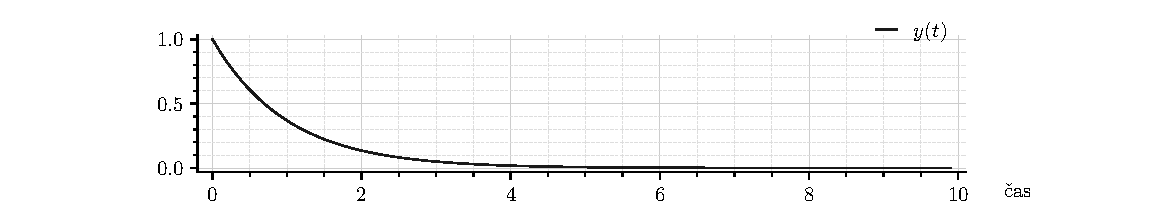
\includegraphics{ICH_SS1R_p1.pdf}
        }

        \figcaption{Impulzná charakteristika statického systému prvého rádu pre $a_0 = 1$ a $b_0 = 1$}
        \label{ICH_SS1R_p1}
    }%vbox

\end{center}



\paragraph{ICH AS1R}

Časová funkcia \eqref{eq:ICH1R} bude impulznou charakteristikou astatického systému prvého rádu ak $a_0 = 0$. Na nasledujúcom obrázku je graf výslednej časovej funkcie

\begin{center}

    \vbox{%
        \makebox[\textwidth][c]{%
        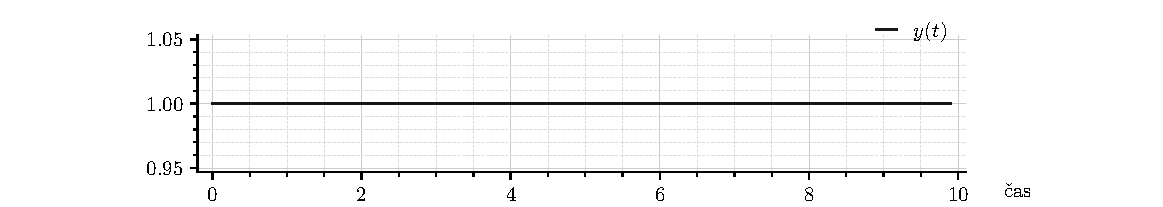
\includegraphics{ICH_AS1R_p1.pdf}
        }

        \figcaption{Impulzná charakteristika statického systému prvého rádu pre $a_0 = 0$ a $b_0 = 1$}
        \label{ICH_AS1R_p1}
    }%vbox

\end{center}




\paragraph{ICH nestabilného systému prvého rádu}

Pre úplnosť uveďme aj prípad, keď $a_0 < 0$, teda systém je nestabilný. Zvoľme $a_0 = -1$. Na nasledujúcom obrázku je graf výslednej časovej funkcie

\begin{center}

    \vbox{%
        \makebox[\textwidth][c]{%
        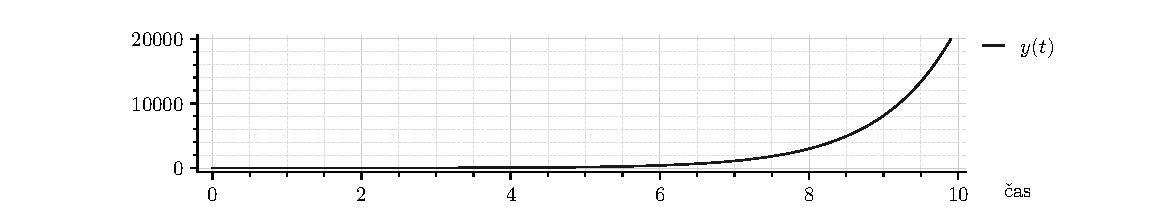
\includegraphics{ICH_unstable1R_p1.pdf}
        }

        \figcaption{Impulzná charakteristika statického systému prvého rádu pre $a_0 = -1$ a $b_0 = 1$}
        \label{ICH_unstable1R_p1}
    }%vbox

\end{center}



\paragraph{Python skript pre vykreslenie grafov impulzných charakteristík}

V tejto časti je prezentovaný skript v programovacom jazyku Python, pomocou ktorého je možné nakresliť vyššie uvedené grafy impulzných charakteristík. Skript je prezentovaný formou Jupyter notebooku a v nasledujúcom sú zobrazené jednotlivé bunky bunky notebooku.


\input{../../PY/jupynotex/tex/MRS07_ICH1Ripynb_2-.tex}






\paragraph{MATLAB: Control System Toolbox}

S využitím \emph{Control System Toolbox} v MATLABe je možné získať ICH príkazom  \lstinline|impulse()|. Samozrejme, najprv je potrebné zadefinovať systém, ktorého ICH nás zaujíma, čo je možné v tomto toolboxe priamo vo forme prenosovej funkcie príkazom  \lstinline|tf()|. Teda:
\begin{lstlisting}[language=Matlab,]
G = tf([1], [1, 1])
impulse(G)
\end{lstlisting}
\noindent
pričom príkaz \lstinline|impulse()| priamo vykreslí aj obrázok.




\paragraph{MATLAB: Simulink}

V Simulinku je napríklad možné realizovať aproximáciu Dirackovho impulzu pomocou bloku \lstinline|Step| s nasledovným nastavením:
\begin{center}

    \makebox[\textwidth][c]{%
	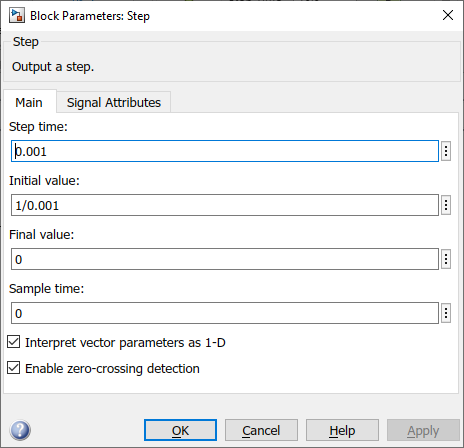
\includegraphics[width=0.68\textwidth]{stepSetup_DiracApprox.png}
	}

	\figcaption{Nastavenie bloku \lstinline|Step|.}
	\label{stepSetup_DiracApprox.png}

\end{center}


Blok je súčasťou schémy:
\begin{center}

    \makebox[\textwidth][c]{%
	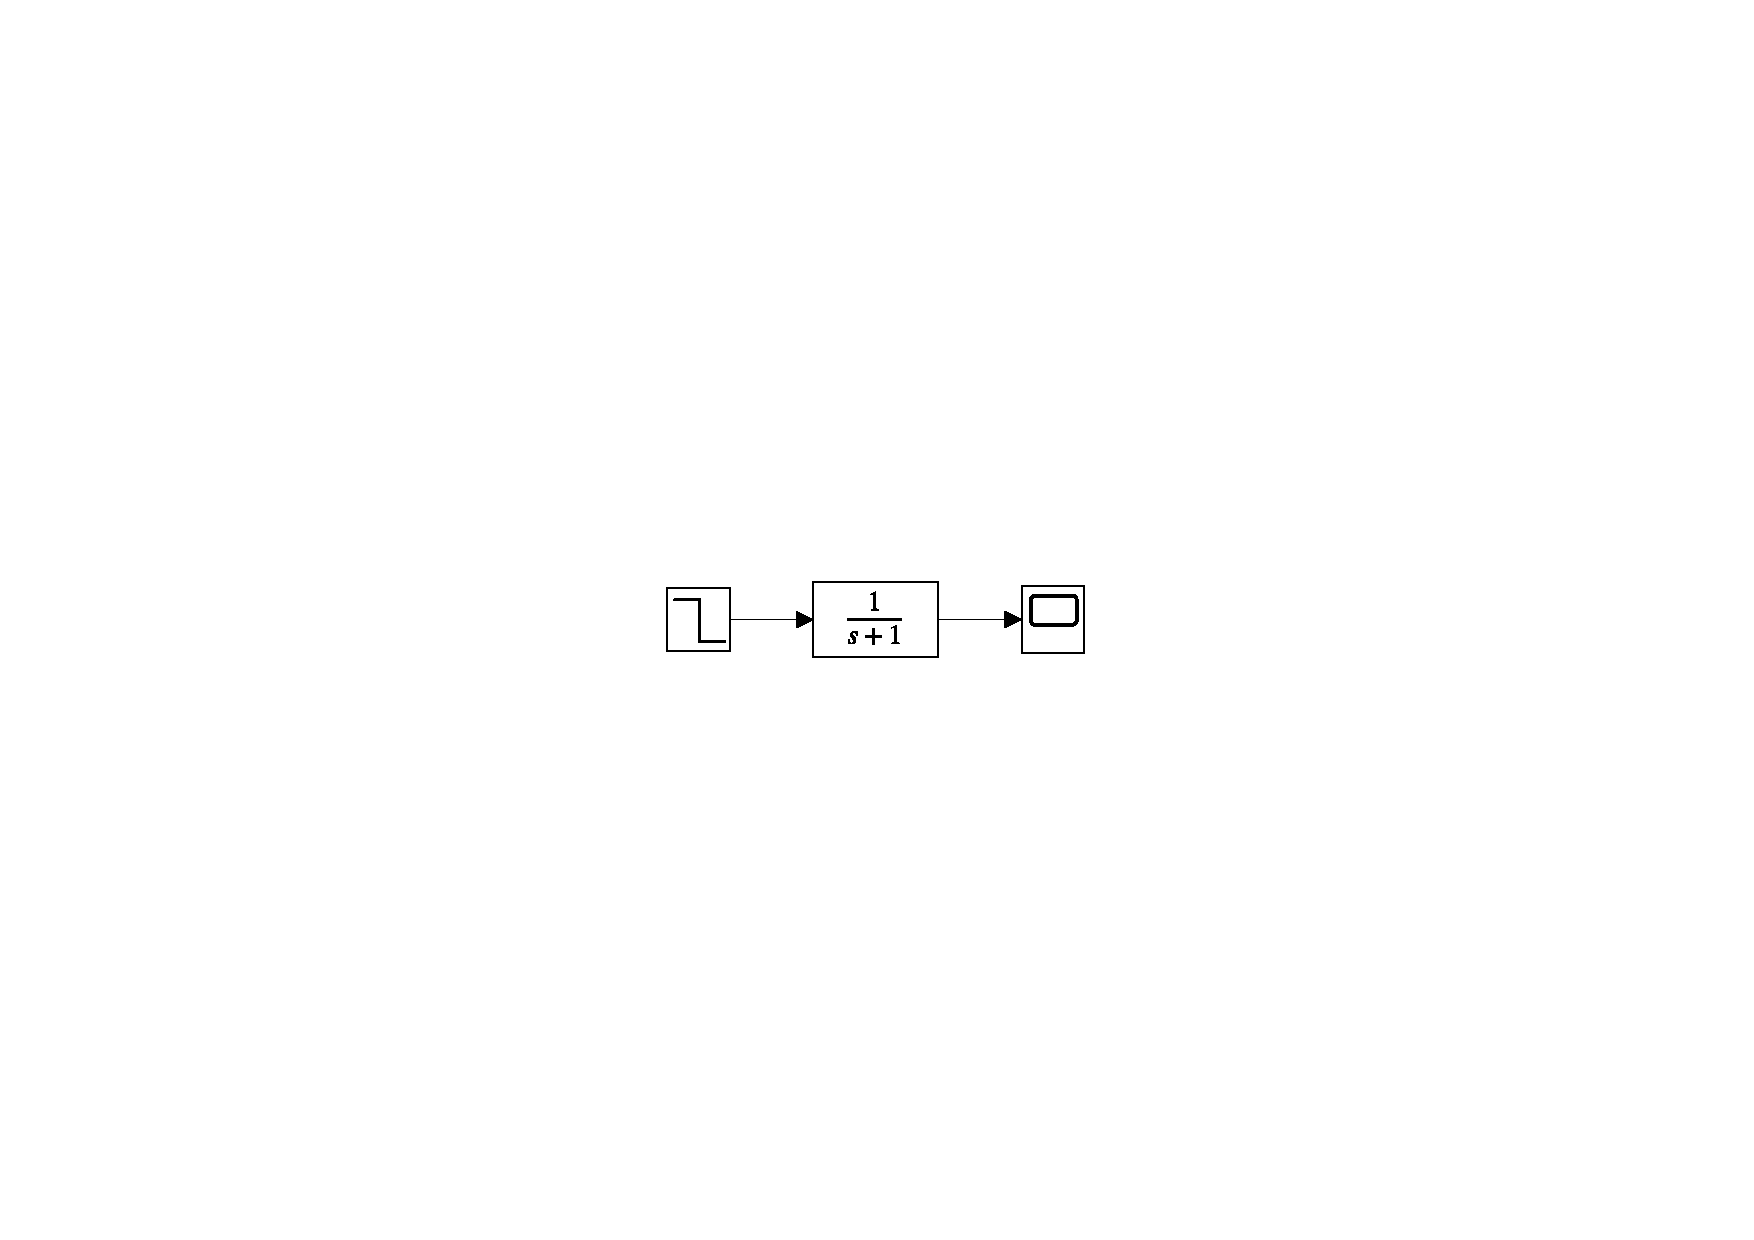
\includegraphics[trim=110mm 95mm 110mm 95mm, clip]{simulinkICHSS1R.pdf}
	}

    \vspace{-5mm}

	\figcaption{Simulačná schéma pre ICH SS1R}
	\label{sim_ICHSS1R}

    \vspace{-1mm}

\end{center}






\subsubsection{Prechodová charakteristika}


Prechodová charakteristika je odpoveď systému na jednotkový skok.

\bigskip

Jednotkový skok je signál, ktorý je nulový pre $t < 0$ a má jednotkovú veľkosť pre $t \geq 0$. Ide o skokovú zmenu v čase $t=0$. Laplaceov obraz jednotkového skoku je $U(s) = \frac{1}{s}$.

Keďže máme k dispozícii matematický opis systému, prechodovú charakteristiku môžeme	nájsť analyticky. Prenosová funkcia systému prvého rádu je \eqref{eq:prvyradprenosovafunkcia}. Laplaceov obraz vstupného signálu je $U(s) = \frac{1}{s}$. Laplaceov obraz výstupného signálu potom bude
\begin{subequations}
\begin{align}
    Y(s) &= G(s) U(s) = \frac{b_0}{s + a_0} \frac{1}{s} \\
    Y(s) &= \frac{b_0}{s(s + a_0)}
\end{align}
\end{subequations}
Pre hľadanie originálu tohto obrazu je výhodné prepísať tento výraz na parciálny zlomok
\begin{subequations}
\begin{align}
    \frac{b_0}{s(s + a_0)} &= \frac{A}{s} + \frac{B}{s + a_0} \\
    b_0 &= A(s + a_0) + B s
\end{align}
\end{subequations}
kde $A$ a $B$ sú neznáme koeficienty. Uvedené platí pre akúkoľvek hodnotu $s$. Pre $s = 0$ dostaneme
\begin{subequations}
\begin{align}
    b_0 &= A a_0 \\
    A &= \frac{b_0}{a_0}
\end{align}
\end{subequations}
Pre $s = -a_0$ dostaneme
\begin{subequations}
\begin{align}
    b_0 &= B (-a_0) \\
    B &= -\frac{b_0}{a_0}
\end{align}
\end{subequations}
Obraz výstupného signálu je teda
\begin{equation}
    Y(s) = \frac{b_0}{a_0} \frac{1}{s} - \frac{b_0}{a_0} \frac{1}{s + a_0}
\end{equation}
a jeho originál
\begin{subequations}
\begin{align}
    y(t) &= \frac{b_0}{a_0} - \frac{b_0}{a_0} e^{-a_0 t} \\
    y(t) &= \frac{b_0}{a_0} \left(1 - e^{-a_0 t}\right)  \label{eq:PCH1Rfull}
\end{align}
\end{subequations}
čo je časová funkcia, ktorá je analytickým vyjadrením prechodovej charakteristiky systému. V uvedenom sme zjavne predpokladali, že $a_0 \neq 0$. 

Ak $a_0 = 0$, potom obraz výstupného signálu je
\begin{subequations}
\begin{align}
    Y(s) &= \frac{b_0}{s^2} \\
    Y(s) &= b_0 \frac{1}{s^2}
\end{align}
\end{subequations}
a jeho originál je
\begin{equation} \label{eq:PCH1Rint}
    y(t) = b_0 t
\end{equation}
čo je časová funkcia, ktorá je analytickým vyjadrením prechodovej charakteristiky systému ak $a_0 = 0$.


Je zrejmé, že pre prechodovú charakteristiku (PCH) je možné rozlišovať kvalitatívne rôzne prípady určené v tomto prípade jediným pólom systému. Pól systému je $s_1 = -a_0$.

V kontexte vyššie uvedeného možno rozlišovať prípady: statický systém prvého rádu (SS1R), astatický systém prvého rádu (AS1R) a nestabilný systém.





\paragraph{PCH SS1R}

Časová funkcia \eqref{eq:PCH1Rfull} bude prechodovou charakteristikou statického systému prvého rádu ak $a_0 > 0$. Zvoľme $a_0 = 1$ a napríklad $b_0 = 1$. Na nasledujúcom obrázku je graf výslednej časovej funkcie

\begin{center}

    \vbox{%
        \makebox[\textwidth][c]{%
        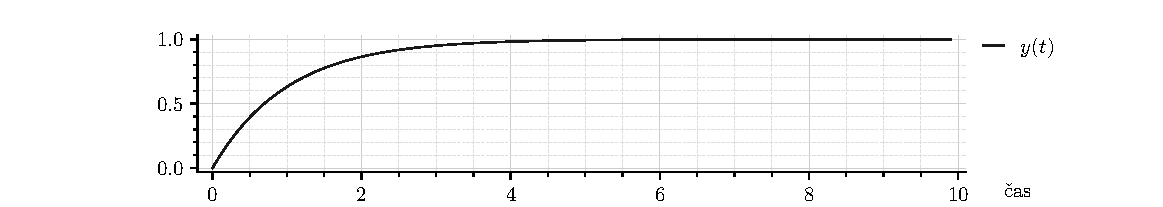
\includegraphics{PCH_SS1R_p1.pdf}
        }

        \figcaption{Prechodová charakteristika statického systému prvého rádu pre $a_0 = 1$ a~$b_0 = 1$}
        \label{PCH_SS1R_p1}
    }%vbox

\end{center}



\paragraph{PCH AS1R}

Časová funkcia \eqref{eq:PCH1Rint} bude prechodovou charakteristikou astatického systému prvého rádu ak $a_0 = 0$. Na nasledujúcom obrázku je graf výslednej časovej funkcie

\begin{center}

    \vbox{%
        \makebox[\textwidth][c]{%
        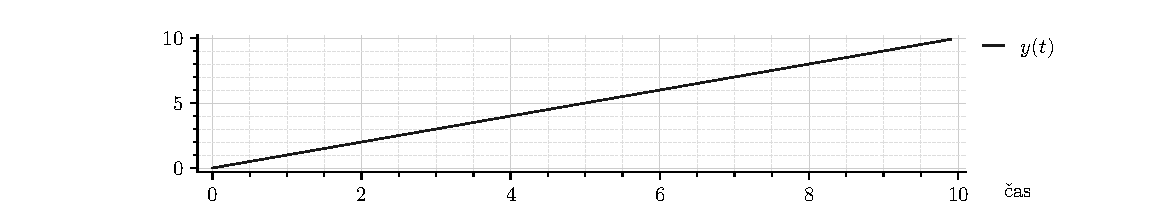
\includegraphics{PCH_AS1R_p1.pdf}
        }

        \figcaption{Prechodová charakteristika astatického systému prvého rádu pre $a_0 = 0$ a~$b_0 = 1$}
        \label{PCH_AS1R_p1}
    }%vbox

\end{center}


\paragraph{PCH nestabilného systému prvého rádu}

Pre úplnosť uveďme aj prípad, keď $a_0 < 0$, teda systém je nestabilný. Zvoľme $a_0 = -1$. Na nasledujúcom obrázku je graf výslednej časovej funkcie

\begin{center}

    \vbox{%
        \makebox[\textwidth][c]{%
        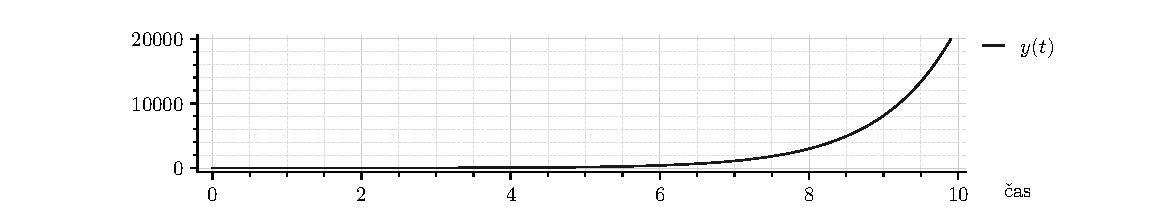
\includegraphics{PCH_unstable1R_p1.pdf}
        }

        \figcaption{Prechodová charakteristika statického systému prvého rádu pre $a_0 = -1$ a~$b_0 = 1$}
        \label{PCH_unstable1R_p1}
    }%vbox

\end{center}



\paragraph{Python skript pre vykreslenie grafov prechodových charakteristík}

V tejto časti je prezentovaný skript v programovacom jazyku Python, pomocou ktorého je možné nakresliť vyššie uvedené grafy prechodových charakteristík. Skript je prezentovaný formou Jupyter notebooku a v nasledujúcom sú zobrazené jednotlivé bunky notebooku.

\input{../../PY/jupynotex/tex/MRS07_PCH1Ripynb_2-.tex}



\paragraph{MATLAB: Control System Toolbox}

S využitím \emph{Control System Toolbox} v MATLABe je možné získať PCH príkazom  \lstinline|step()|. Samozrejme, najprv je potrebné zadefinovať systém, ktorého PCH nás zaujíma, čo je možné v tomto toolboxe priamo vo forme prenosovej funkcie príkazom  \lstinline|tf()|. Teda:
\begin{lstlisting}[language=Matlab,]
G = tf([1], [1, 1])
step(G)
\end{lstlisting}
\noindent
pričom príkaz \lstinline|step()| sa postará o časové nastavenie simulácie (nájde vhodné nastavenie pre ODE solver atď) a priamo vykreslí aj obrázok.


\paragraph{MATLAB: Simulink}

Simulink priamo ponúka prácu s prenosovými funkciami a teda za užívateľa vykoná prevod do opisu v stavovom priestore a vykoná numerickú simuláciu. Pre tento prípad by schéma v simulinku vyzerala nasledovne:

\begin{center}

    \makebox[\textwidth][c]{%
	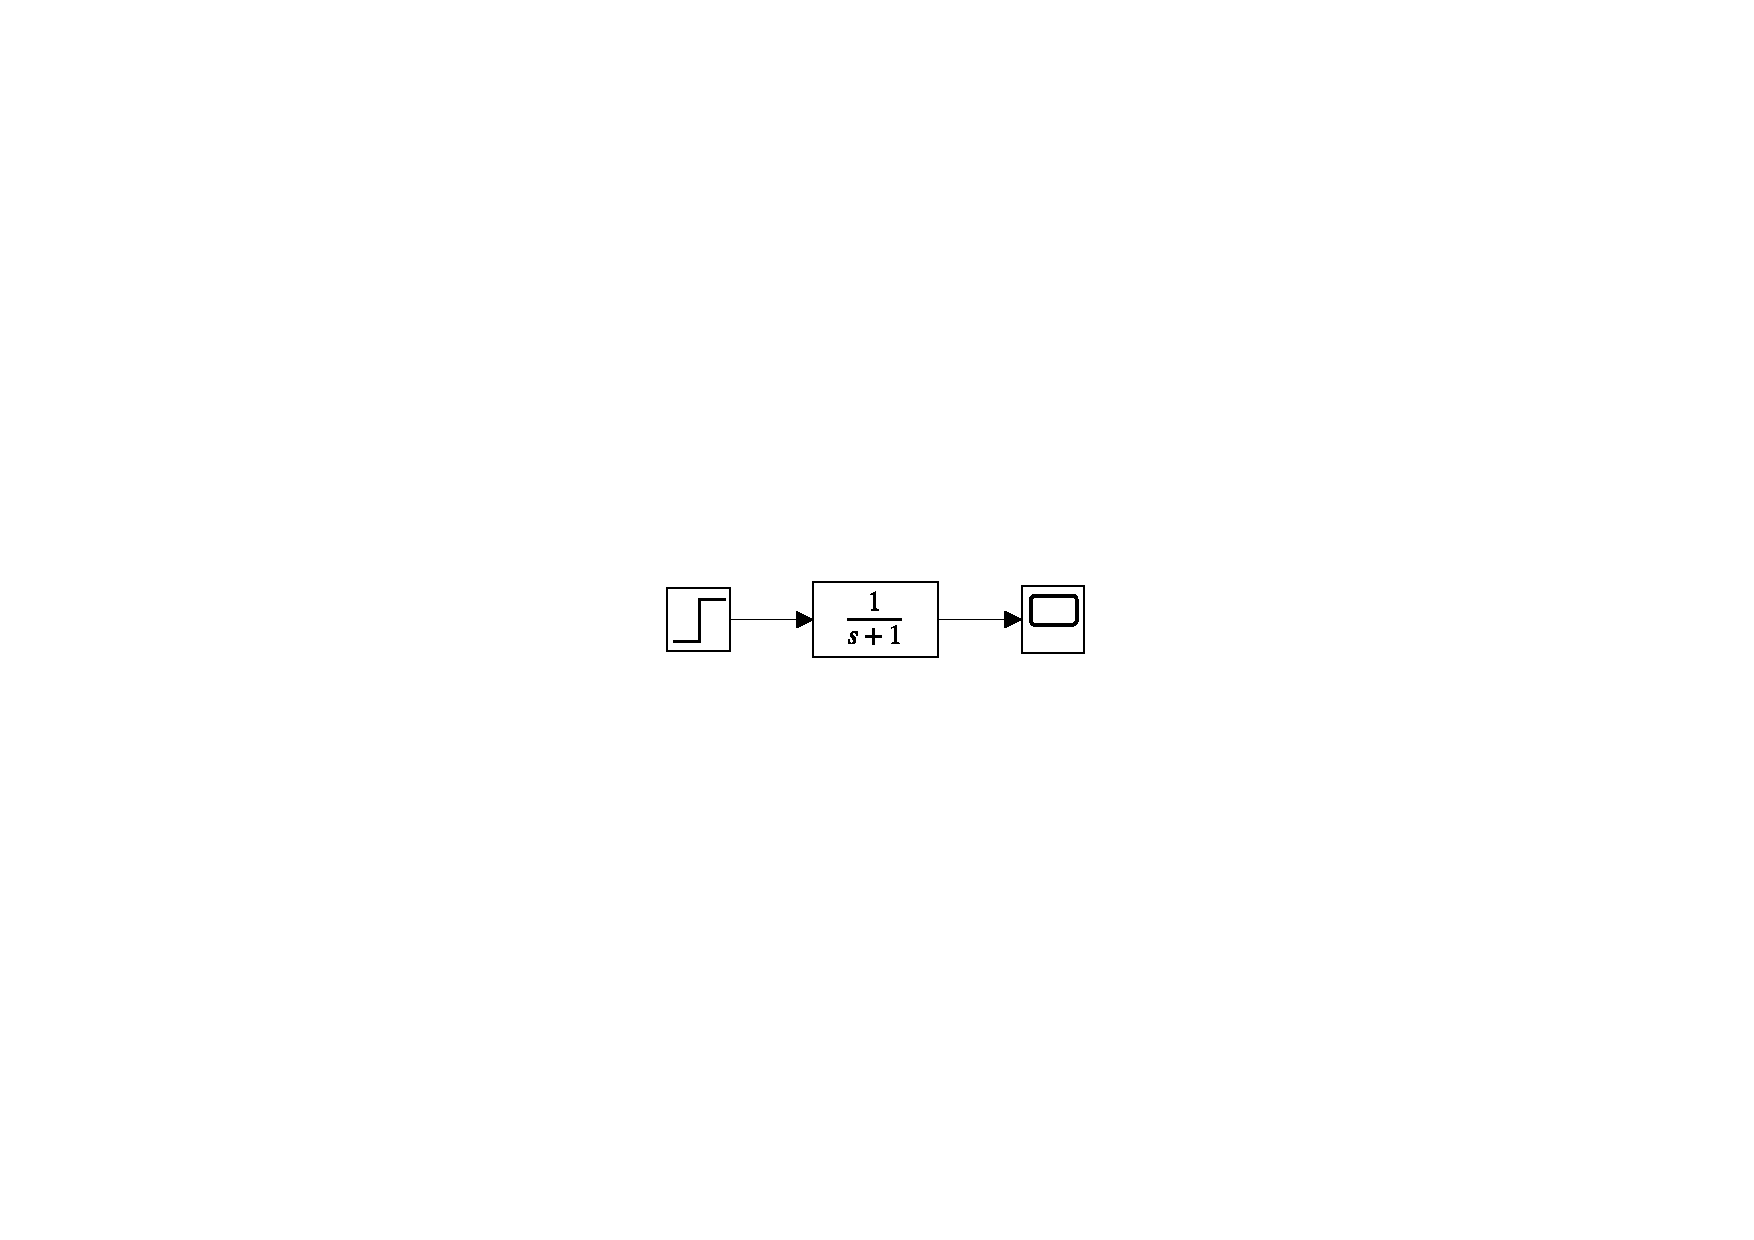
\includegraphics[trim=110mm 95mm 110mm 95mm, clip]{simulinkPCHSS1R.pdf}
	}

    \vspace{-5mm}

	\figcaption{Simulačná schéma pre PCH SS1R}
	\label{sim_PCHSS1R}

    \vspace{-1mm}

\end{center}

V bloku \lstinline|Step| je v tomto prípade nastavený skok v~čase $0$~z~hodnoty $0$~na hodnotu~$1$.





\subsection{Systém nultého rádu}

Stupeň polynómu $A(s)$ môže byť aj $n = 0$. Potom hovoríme o systéme nultého rádu. Prenosová funkcia v tomto prípade je (aj vzhľadom na kauzálnosť, aj vzhľadom na pozitívnu reálnosť)
\begin{align}
    G(s) = \frac{b_0}{a_0}
\end{align}

Hovoriť v tomto prípade o dynamike v podstate nie je možné. Ide tu vo všeobecnosti o zosilňovač, ktorého statické zosilnenie je
\begin{align}
    \frac{y(\infty)}{u(\infty)} = \frac{b_0 }{a_0}
\end{align}
Takýto systém má len statické vlastnosti (statické zosilnenie -- sklon prevodovej charakteristiky). O~dynamických vlastnostiach, v~zmysle astatizmu, stability a~prechodovej charakteristiky tu nemá význam hovoriť.






\subsection{Systém druhého rádu}


\subsubsection{Prenosová funkcia}

Ak stupeň polynómu $A(s)$ je $n = 2$, potom hovoríme, že systém je druhého rádu. Pre kauzálnosť a aj pre pozitívnu reálnosť tu uvažujeme $m<n$ a tak vo všeobecnosti
\begin{align} \label{typ2radtf}
    G(s) = \frac{b_1 s + b_0}{s^2 + a_1 s + a_0}
\end{align}
kde je $A(s)$ bez straty na všeobecnosti uvedený ako monický polynóm.

Obdobne, prenosovou funkciou druhého rádu sú:
\begin{subequations}
    \begin{align}
        G(s) &= \frac{b_0}{s^2 + a_1 s + a_0} \\
        G(s) &= \frac{b_1 s}{s^2 + a_1 s + a_0}
    \end{align}
\end{subequations}



\subsubsection{Diferenciálna rovnica}

Nech je systém daný v tvare prenosovej funkcie
\begin{equation}
    G(s) = \frac{Y(s)}{U(s)}
\end{equation}
kde $Y(s)$ je Laplaceov obraz výstupného signálu a $U(s)$ je Laplaceov obraz vstupného signálu. Nech cieľom je prepis do tvaru diferenciálnej rovnice, potom
\begin{subequations}
    \begin{align}
        Y(s) &= G(s) U(s) = \frac{b_1 s + b_0}{s^2 + a_1 s + a_0} U(s) \\
        (s^2 + a_1 s + a_0) Y(s) &= (b_1 s + b_0) U(s) \\
        s^2 Y(s) + a_1 s Y(s) + a_0 Y(s) &= b_1 s U(s) + b_0 U(s) \\
        s^2 Y(s) &= - a_1 s Y(s) - a_0 Y(s) + b_1 s U(s) + b_0 U(s) 
    \end{align}
\end{subequations}
a teda diferenciálna rovnica je
\begin{equation} \label{difrovnica2rad}
    \ddot y(t)  =  - a_1 \dot y(t) - a_0 y(t) + b_1 \dot u(t) + b_0 u(t)
\end{equation}

Prepis opačným smerom, z dif. rovnice na prenosovú funkciu, je samozrejme štandardné aplikovanie Laplaceovej transformácie na rovnicu \eqref{difrovnica2rad} pri nulových začiatočných podmienkach.







\subsubsection{Opis systému v stavovom priestore}

V stavovom priestore je potrebné zaviesť stavový vektor $x(t) \in \mathbb R^n$. Vo všeobecnosti je opis lineárneho systému v stavovom priestore v tvare
\begin{subequations}
\begin{align}
    \dot x(t) &= A x(t) + b u(t) \\
    y(t) &= c^\naT x(t) 
\end{align}
\end{subequations}
kde $A \in \mathbb R^{n \times n}$, $b \in \mathbb R^n$ a $c \in \mathbb R^n$ sú matica a vektory a ide o parametre systému.

Pri stanovení vektora $x(t)$ ide vo všeobecnosti o prepis diferenciálnej rovnice vyššieho rádu na sústavu rovníc prvého rádu. Vzniknú tak nové signály, ktoré sú neznámymi v sústave rovníc prvého rádu a sú prvkami stavového vektora $x(t)$.



\paragraph{Príkladný postup pre voľbu stavových veličín}

Prevod z prenosovej funkcie na stavový opis nie je jednoznačný. Záleží na voľbe stavových veličín (stavového priestoru). Tu si dovolíme uviesť voľbu stavových veličín tak, že výsledkom je opis systému v tzv. normálnej forme riaditeľnosti.

Prenosová funkcia systému, ktorou sa tu zaoberáme, je v tvare
\begin{align} \label{tfVseob01}
	\frac{Y(s)}{U(s)} = \frac{b_1 s + b_0}{ s^2 + a_1 s + a_0}
\end{align}
Otázka je ako túto prenosovú funkciu previesť na opis v stavovom priestore - ako zvoliť stavové veličiny.

Pre prípad, keď je v čitateli len konštanta (systém nemá nuly), je voľba stavových veličín značne intuitívna. Preto napíšme prenosovú funkciu \eqref{tfVseob01} ako dve prenosové funkcie v sérii nasledovne
\begin{align}
	\frac{Z(s)}{U(s)} &= \frac{1}{ s^2 + a_1 s + a_0} \label{tfVseob02a} \\
    \frac{Y(s)}{Z(s)} &= b_1 s + b_0 \label{tfVseob02b}
\end{align}
kde sme zaviedli pomocnú veličinu $Z(s)$, ktorá je obrazom $z(t)$. Zjavne platí
\begin{align}
    \frac{Y(s)}{U(s)} = \frac{Y(s)}{Z(s)} \frac{Z(s)}{U(s)}
\end{align}
alebo explicitnejšie:
\begin{align}
    \frac{Y(s)}{U(s)} = \left( b_1 s + b_0 \right) \frac{1}{ s^2 + a_1 s + a_0}
\end{align}

Mimochodom, prenosová funkcia \eqref{tfVseob02b} je z matematického hľadiska korektná akurát v čitateli je polynóm stupňa $1$ a v menovateli polynóm stupňa $0$, čo napríklad znamená, že ide o nekauzálny systém a teda sama o sebe by prenosová funkcia \eqref{tfVseob02b} nebola vhodným modelom reálneho fyzikálneho systému.

Prvú prenosovú funkciu \eqref{tfVseob02a} možno prepísať na diferenciálnu rovnicu druhého rádu v tvare
\begin{align} \label{origdifeqnz}
	\ddot z(t) + a_1 \dot z(t) + a_0 z(t) = u(t)
\end{align}

Túto je možné previesť na sústavu diferenciálnych rovníc prvého rádu - voľbou stavových veličín. Napríklad nech
\begin{align}
	x_1(t) = z(t)
\end{align}
kde $x_1(t)$ je prvá stavová veličina. Potom platí
\begin{align}
	\dot x_1(t) = \dot z(t)
\end{align}
Druhú stavovú veličinu zvoľme
\begin{align}
	x_2(t) = \dot z(t)
\end{align}
a teda
\begin{align} \label{zardrufdifr}
	\dot x_2(t) = \ddot z(t)
\end{align}
V tomto bode môžeme ľahko písať
\begin{align}
	\dot x_1(t) &= x_2(t)
\end{align}
To je prvá diferenciálna rovnica! Obsahuje len novo zavedené stavové veličiny ($x_1(t)$ a~$x_2(t)$). Druhá diferenciálna rovnica je vlastne \eqref{zardrufdifr}. Avšak, vieme signál $\ddot z(t)$ vyjadriť len pomocou novo zavedených stavových veličín? Vieme. Z \eqref{origdifeqnz} je zrejmé, že
\begin{align}
	\ddot z(t) = - a_1 \dot z(t) - a_0 z(t) + u(t) = - a_1 x_2(t) - a_0 x_1(t) + u(t)
\end{align}
takže \eqref{zardrufdifr} je
\begin{align}
	\dot x_2(t) =  - a_1 x_2(t) - a_0 x_1(t) + u(t)
\end{align}
a to je druhá diferenciálna rovnica\ldots

\noindent
Obe rovnice spolu:
\begin{align}
    \dot x_1(t) &= x_2(t) \\
	\dot x_2(t) &=  - a_1 x_2(t) - a_0 x_1(t) + u(t)
\end{align}
V maticovom zápise:
\begin{align}
	\begin{bmatrix}
    	  \dot x_1(t) \\
		  \dot x_2(t)
 	\end{bmatrix}
	&=
	\begin{bmatrix}
    	0 & 1 \\
    	- a_0 & - a_1
  	\end{bmatrix}
    \begin{bmatrix}
    	  x_1(t) \\
		  x_2(t)
 	\end{bmatrix}
    +
    \begin{bmatrix}
    	  0 \\
		  1
 	\end{bmatrix}
    u(t)
\end{align}

Vráťme sa k prenosovej funkcii \eqref{tfVseob02b}. Túto možno napísať ako diferenciálnu rovnicu v tvare
\begin{align} \label{difrov2}
    y(t) = b_1 \dot z(t) + b_0 z(t)
\end{align}
Avšak, my sme už urobili voľbu takú, že $\dot z(t) = x_2(t)$ a $z(t)= x_1(t)$. Takže diferenciálnu rovnicu \eqref{difrov2} môžme písať ako
\begin{align}
    y(t) = b_1 x_2(t) + b_0 x_1(t)
\end{align}
alebo v maticovom tvare
\begin{align}
	y(t)
	&=
	\begin{bmatrix}
    	b_0 & b_1 \\
  	\end{bmatrix}
    \begin{bmatrix}
    	  x_1(t) \\
		  x_2(t)
 	\end{bmatrix}
\end{align}

Celý systém s novo zavedenými stavovými veličinami teda je v tvare
\begin{align}
	\begin{bmatrix}
    	  \dot x_1(t) \\
		  \dot x_2(t)
 	\end{bmatrix}
	&=
	\begin{bmatrix}
    	0 & 1 \\
    	- a_0 & - a_1
  	\end{bmatrix}
    \begin{bmatrix}
    	  x_1(t) \\
		  x_2(t)
 	\end{bmatrix}
    +
    \begin{bmatrix}
    	  0 \\
		  1
 	\end{bmatrix}
    u(t)
    \\
    y(t)
    &=
    \begin{bmatrix}
        b_0 & b_1 \\
    \end{bmatrix}
    \begin{bmatrix}
          x_1(t) \\
          x_2(t)
    \end{bmatrix}
\end{align}
Ak označíme stavový vektor ako $x(t) = \begin{bmatrix} x_1(t) & x_2(t) \end{bmatrix}^\naT$, potom je systém v známom tvare
\begin{subequations} \label{susDifRovnicPreODE}
    \begin{align}
    	\dot x(t) &= A x(t) + b u(t) \\
        y(t) &= c^\naT x(t)
    \end{align}
\end{subequations}
kde
\begin{subequations}
\begin{align}
    A &=
    \begin{bmatrix}
    	0 & 1 \\
    	- a_0 & - a_1
  	\end{bmatrix}
    \\
    b &=
    \begin{bmatrix}
    	  0 \\
          1
 	\end{bmatrix}
    \\
    c &=
    \begin{bmatrix}
        b_0 \\ b_1 
    \end{bmatrix}
\end{align}
\end{subequations}







\paragraph{Následné príklady priameho stanovenia opisu systému v stavovom priestore}

Vidíme, že ak máme prenosovú funkciu v tvare
\begin{align} \label{tfVseob02}
	\frac{Y(s)}{U(s)} = \frac{b_1 s + b_0}{ s^2 + a_1 s + a_0}
\end{align}
tak opis systému v stavovom priestore je v tvare
\begin{subequations}
\begin{align}
    \dot x(t)
    &=
    \begin{bmatrix}
    	0 & 1 \\
    	- a_0 & - a_1
  	\end{bmatrix}
    x(t)
    +
    \begin{bmatrix}
    	  0 \\
          1
 	\end{bmatrix}
    u(t)
    \\
    y(t)
    &=
    \begin{bmatrix}
        b_0 & b_1 \\
    \end{bmatrix}
    x(t)
\end{align}
\end{subequations}
kde samozrejme $x(t) \in \mathbb R^2$ je stavový vektor. 
Obdobne, ak máme prenosovú funkciu v~tvare
\begin{align} 
	\frac{Y(s)}{U(s)} = \frac{b_0}{ s^2 + a_1 s + a_0}
\end{align}
tak opis systému v stavovom priestore je v tvare
\begin{subequations}
\begin{align}
    \dot x(t)
    &=
    \begin{bmatrix}
    	0 & 1 \\
    	- a_0 & - a_1
  	\end{bmatrix}
    x(t)
    +
    \begin{bmatrix}
    	  0 \\
          1
 	\end{bmatrix}
    u(t)
    \\
    y(t)
    &=
    \begin{bmatrix}
        b_0 & 0 \\
    \end{bmatrix}
    x(t)
\end{align}
\end{subequations}
čo je možné zapísať aj v tvare
\begin{subequations}
    \begin{align}
        \dot x(t)
        &=
        \begin{bmatrix}
            0 & 1 \\
            - a_0 & - a_1
          \end{bmatrix}
        x(t)
        +
        \begin{bmatrix}
              0 \\
              b_0
         \end{bmatrix}
        u(t)
        \\
        y(t)
        &=
        \begin{bmatrix}
            1 & 0 \\
        \end{bmatrix}
        x(t)
\end{align}
\end{subequations}
pretože sme len zmenili miesto, kde koeficient $b_0$ násobí zodpovedajúci signál. Je jedno, či je to na vstupe, alebo na výstupe. 

Pre úplnosť, ak máme prenosovú funkciu v tvare
\begin{align} 
	\frac{Y(s)}{U(s)} = \frac{b_1 s }{ s^2 + a_1 s + a_0}
\end{align}
tak opis systému v stavovom priestore je v tvare
\begin{subequations}
\begin{align}
    \dot x(t)
    &=
    \begin{bmatrix}
    	0 & 1 \\
    	- a_0 & - a_1
  	\end{bmatrix}
    x(t)
    +
    \begin{bmatrix}
    	  0 \\
          1
 	\end{bmatrix}
    u(t)
    \\
    y(t)
    &=
    \begin{bmatrix}
        0 & b_1 \\
    \end{bmatrix}
    x(t)
\end{align}
\end{subequations}
Ešte iným príkladom by mohla byť prenosová funkcia v tvare
\begin{align} 
	\frac{Y(s)}{U(s)} = \frac{b_0 }{ s^2 +  a_0}
\end{align}
a opis systému v stavovom priestore by bol
\begin{subequations}
    \begin{align}
        \dot x(t)
        &=
        \begin{bmatrix}
            0 & 1 \\
            0 & - a_1
          \end{bmatrix}
        x(t)
        +
        \begin{bmatrix}
              0 \\
              1
         \end{bmatrix}
        u(t)
        \\
        y(t)
        &=
        \begin{bmatrix}
            b_0 & 0 \\
        \end{bmatrix}
        x(t)
\end{align}
\end{subequations}






\paragraph{Z opisu v stavovom priestore na prenosovú funkciu}

Majme systém daný v stavovom priestore v tvare
\begin{subequations} \label{difRovSustavaKPrevodu}
    \begin{align} 
        \dot x(t) &= A x(t) + b u(t) \label{difRovSustavaKPrevodua}\\
        y(t) &= c^\naT x(t) 
    \end{align}
\end{subequations}
kde stavový vektor $x(t) \in \mathbb R^n$, $A \in \mathbb R^{n \times n}$, $b \in \mathbb R^n$ a $c \in \mathbb R^n$ sú matica a vektory a ide o parametre systému. 

Rovnica \eqref{difRovSustavaKPrevodua} je takpovediac vektorovou diferenciálnou rovnicou, čím tu myslíme, že neznámou je vektor $x(t)$ obsahujúci signály (stavové veličiny).

Na rovnice \eqref{difRovSustavaKPrevodu} je možné aplikovať Laplaceovú transformáciu. Potom pri nulových začiatočných podmienkach, pretože našim cieľom je prenosová funkcia, je možné písať
\begin{subequations}
    \begin{align}
        s I X(s) &= A X(s) + b U(s) \label{SRovSustavaKPrevodua} \\
        Y(s) &= c^\naT X(s) \label{SRovSustavaKPrevodub}
    \end{align}
\end{subequations}
kde $I$ je jednotková matica rovnakého rozmeru ako $A$ a $s$ je Laplaceov operátor. Výraz $s I$ je potom matica, ktorá má na diagonále Laplaceove operátory. $X(s)$ je samozrejme vektor, ktorý obsahuje Laplaceove obrazy stavových veličín.

Prenosová funkcia je pomerom obrazov výstupu a vstupu. Je vhodné začať rovnicou \eqref{SRovSustavaKPrevodua} a vyjadriť pomer obrazov $X(s)$ a $U(s)$. Môžeme písať
\begin{align}
    s I X(s) &= A X(s) + b U(s) \\
    s I X(s) - A X(s) &= b U(s)
\end{align}
pričom rozmery jednotlivých matíc a vektorov boli zachované. Potom
\begin{align}
    (s I - A) X(s) &= b U(s)
\end{align}
kde $(s I - A)$ je matica. Je potrebné osamostatniť $X(s)$. Celú rovnicu je preto potrebné vynásobiť zľava inverznou maticou k matici $(s I - A)$, teda maticou $(s I - A)^{-1}$.
\begin{align}
    (s I - A)^{-1} (s I - A) X(s) &= (s I - A)^{-1} b U(s) \\
    X(s) &= (s I - A)^{-1} b U(s)
\end{align}
Teraz je možné dosadiť za $X(s)$ do rovnice \eqref{SRovSustavaKPrevodub}, teda
\begin{align}
    Y(s) &= c^\naT X(s) \\
    Y(s) &= c^\naT (s I - A)^{-1} b U(s)
\end{align}
Pomer $Y(s)$ a $U(s)$ je
\begin{align}
    \frac{Y(s)}{U(s)} = c^\naT (s I - A)^{-1} b
\end{align}
a teda prenosová funkcia je
\begin{align}
    G(s) = c^\naT (s I - A)^{-1} b
\end{align}

Majme konkrétny prípad, keď systém je daný v stavovom priestore v tvare
\begin{subequations}
    \begin{align}
        \dot x(t)
        &=
        \begin{bmatrix}
            0 & 1 \\
            - a_0 & - a_1
          \end{bmatrix}
        x(t)
        +
        \begin{bmatrix}
              0 \\
              1
         \end{bmatrix}
        u(t)
        \\
        y(t)
        &=
        \begin{bmatrix}
            b_0 & b_1 \\
        \end{bmatrix}
        x(t)
\end{align}
\end{subequations}
a teda $A = \begin{bmatrix} 0 & 1 \\ - a_0 & - a_1 \end{bmatrix}$, $b = \begin{bmatrix} 0 \\ 1 \end{bmatrix}$ a $c = \begin{bmatrix} b_0 \\ b_1 \end{bmatrix}$. Stanovme maticu $(s I - A)$:
\begin{align}
    (s I - A) &=
    \begin{bmatrix}
        s & 0 \\
        0 & s
    \end{bmatrix}
    -
    \begin{bmatrix}
        0 & 1 \\
        - a_0 & - a_1
    \end{bmatrix}
    =
    \begin{bmatrix}
        s & -1 \\
        a_0 & s + a_1
    \end{bmatrix}
\end{align}
Jej inverzia je
\begin{align}
\begin{aligned}
    (s I - A)^{-1} &=
    \begin{bmatrix}
        s & -1 \\
        a_0 & s + a_1
    \end{bmatrix}^{-1}
    =
    \frac{1}{(s + a_1)s - (-a_0)}
    \begin{bmatrix}
        s + a_1 & 1 \\
        -a_0 & s
    \end{bmatrix} \\
    &=
    \frac{1}{s^2 + a_1s + a_0}
    \begin{bmatrix}
        s + a_1 & 1 \\
        -a_0 & s
    \end{bmatrix} \\
    &=
    \begin{bmatrix}
        \frac{s + a_1}{s^2 + a_1s + a_0} & \frac{1}{s^2 + a_1s + a_0} \\
        \frac{-a_0}{s^2 + a_1s + a_0} & \frac{s}{s^2 + a_1s + a_0}
    \end{bmatrix}
\end{aligned}
\end{align}
Vynásobme sprava vektorom $b$
\begin{align}
    (s I - A)^{-1} b &=
    \begin{bmatrix}
        \frac{s + a_1}{s^2 + a_1s + a_0} & \frac{1}{s^2 + a_1s + a_0} \\
        \frac{-a_0}{s^2 + a_1s + a_0} & \frac{s}{s^2 + a_1s + a_0}
    \end{bmatrix}
    \begin{bmatrix}
        0 \\ 1
    \end{bmatrix}
    =
    \begin{bmatrix}
        \frac{1}{s^2 + a_1s + a_0} \\
        \frac{s}{s^2 + a_1s + a_0}
    \end{bmatrix}
\end{align}
a následne zľava vektorom $c^\naT$
\begin{align}
    c^\naT (s I - A)^{-1} b &=
    \begin{bmatrix}
        b_0 & b_1
    \end{bmatrix}
    \begin{bmatrix}
        \frac{1}{s^2 + a_1s + a_0} \\
        \frac{s}{s^2 + a_1s + a_0}
    \end{bmatrix}
    =
    b_0 \frac{1}{s^2 + a_1s + a_0} + b_1 \frac{s}{s^2 + a_1s + a_0}
\end{align}
a po úprave
\begin{align}
    c^\naT (s I - A)^{-1} b &=
    \frac{b_0 + b_1 s}{s^2 + a_1s + a_0} 
\end{align}
je prenosová funkcia v konkrétnom uvažovanom prípade.











\paragraph{Z opisu v stavovom priestore na diferenciálnu rovnicu}

Majme systém daný v stavovom priestore v tvare
\begin{align}
	\begin{bmatrix}
    	  \dot x_1(t) \\
		  \dot x_2(t)
 	\end{bmatrix}
	&=
	\begin{bmatrix}
    	0 & 1 \\
    	- a_0 & - a_1
  	\end{bmatrix}
    \begin{bmatrix}
    	  x_1(t) \\
		  x_2(t)
 	\end{bmatrix}
    +
    \begin{bmatrix}
    	  0 \\
		  1
 	\end{bmatrix}
    u(t)
    \\
    y(t)
    &=
    \begin{bmatrix}
        b_0 & b_1 \\
    \end{bmatrix}
    \begin{bmatrix}
          x_1(t) \\
          x_2(t)
    \end{bmatrix}
\end{align}
Nech cieľ je prepísať túto sústavu diferenciálnych rovníc na jednu sústavu rovníc vyššieho rádu. V takom prípade je možné pozerať sa na výstupný signál $y(t)$ ako na neznámu v dif. rovnici vyššieho rádu. Sústava rovníc vyzerá nasledovne:
\begin{align}
    \dot x_1(t) &= x_2(t) \label{pr_prva}\\
    \dot x_2(t) &= - a_1 x_2(t) - a_0 x_1(t) + u(t) \label{pr_druha}\\
    y(t) &= b_0 x_1(t) + b_1 x_2(t) \label{pr_tretia}
\end{align}
Napríklad rovnicu \eqref{pr_druha} zderivujme a dosaďme za $\dot x_1(t)$ z prvej rovnice \eqref{pr_prva}
\begin{align}
    \ddot x_2(t) &= - a_1 \dot x_2(t) - a_0 \dot x_1(t) + \dot u(t) \\
    \ddot x_2(t) &= - a_1 \dot x_2(t) - a_0 x_2(t) + \dot u(t) \label{92}
\end{align}
Z rovnice \eqref{pr_tretia} plynie
\begin{align}
    x_2(t) &= \frac{1}{b_1} y(t)  + \frac{b_0}{b_1}  x_1(t) \label{93} \\
    \dot x_2(t) &= \frac{1}{b_1} \dot y(t)  + \frac{b_0}{b_1}  \dot x_1(t) = \frac{1}{b_1} \dot y(t) + \frac{b_0}{b_1}  x_2(t)  \label{94}
\end{align}
a
\begin{subequations} \label{95}
    \begin{align}
        \ddot x_2(t) &= \frac{1}{b_1} \ddot y(t) + \frac{b_0}{b_1} \dot x_2(t) \\
        &= \frac{1}{b_1} \ddot y(t) + \frac{b_0}{b_1} \left( - a_1 x_2(t) - a_0 x_1(t) + u(t) \right) \\
        &= \frac{1}{b_1} \ddot y(t) - \frac{b_0 a_1}{b_1} x_2(t) - \frac{b_0 a_0}{b_1} x_1(t) + \frac{b_0}{b_1} u(t)
    \end{align} 
\end{subequations}
Výsledky \eqref{93} a \eqref{94} a \eqref{95} je možné dosadiť do \eqref{92}, teda
\begin{align}
    &
    \begin{aligned}
    & 
    \frac{1}{b_1} \ddot y(t) - \frac{b_0 a_1}{b_1} x_2(t) - \frac{b_0 a_0}{b_1} x_1(t) + \frac{b_0}{b_1} u(t) 
    \\&
    = - a_0 \left( \frac{1}{b_1} y(t)  + \frac{b_0}{b_1}  x_1(t) \right) - a_1 \left( \frac{1}{b_1} \dot y(t) + \frac{b_0}{b_1}  x_2(t) \right) + \dot u 
    \end{aligned} \\
    &
    \begin{aligned}
    &
    \frac{1}{b_1} \ddot y(t) - \frac{b_0 a_1}{b_1} x_2(t) - \frac{b_0 a_0}{b_1} x_1(t) + \frac{b_0}{b_1} u(t)
    \\&
    = -  \frac{a_0}{b_1}  y(t) -  \frac{ a_0 b_0}{b_1}  x_1(t) -  \frac{a_1}{b_1} \dot y(t) -  \frac{a_1 b_0}{b_1}  x_2(t) + \dot u
    \end{aligned}
\end{align}
a teda
\begin{align}
    \frac{1}{b_1} \ddot y(t)  + \frac{b_0}{b_1} u(t) &= -  \frac{a_0}{b_1}  y(t)  -  \frac{a_1}{b_1} \dot y(t)  + \dot u \\
    \ddot y(t)  + b_0 u(t) &= -  a_0 y(t)  -  a_1 \dot y(t)  + b_1 \dot u \\
    \ddot y(t)  &= -  a_1 \dot y(t)  -  a_0 y(t)  + b_1 \dot u(t) + b_0 u(t)
\end{align}







\subsubsection{Stabilita}

Stabilita systému je daná koreňmi charakteristického polynómu $A(s)$, v tomto prípade
\begin{align}
    A(s) = s^2 + a_1 s + a_0
\end{align}
Tento polynóm má dva korene. Môžu to byť:
\begin{itemize}[leftmargin=0pt, labelsep=3mm, itemsep=0pt]
    \item dve rôzne reálne čísla (imaginárna časť čísla je nulová),
    \item jedno reálne číslo, ktoré je dvojnásobným koreňom,
    \item alebo dve komplexné čísla, ktoré sú však navzájom komplexne združené.
\end{itemize}
V každom prípade však platí, že systém je stabilný vtedy, a len vtedy, ak reálne časti pólov sú záporné (v ľavej polrovine komplexnej roviny).

Ak aspoň jeden koreň leží na imaginárnej osi (reálna časť koreňa je nulová), potom hovoríme, že systém je na hranici stability.

Ak aspoň jeden koreň má reálnu časť kladnú, potom je systém nestabilný.








\subsubsection{Statické zosilnenie a astatizmus}

\paragraph{Statické zosilnenie}

Uvažujme systém, ktorý nie je nestabilný a žiadny z pólov systému nie je nulový. Takýto systém je možné nazvať statickým, pretože pri ustálenom vstupe sa ustáli aj výstup. V tomto prípade máme systém druhého rádu a teda hovoríme o \emph{statickom systéme druhého ráu}, skratka SS2R. 

Pre takýto systém je možné určiť jeho statické zosilnenie. Statické zosilnenie je pomer výstupu ku vstupu v ustálenom stave.

V ustálenom stave sa signály nemenia, to znamená, že ich časové derivácie sú nulové. Všimnime si diferenciálnu rovnicu \eqref{difrovnica2rad}. 
V ustálenom stave je $\dot y(\infty) = 0$, kde $\infty$ symbolizuje čas, v ktorom sú už signály ustálené. Rovnako aj $\ddot y(\infty) = 0$ a $\dot u(\infty) = 0$ a teda
\begin{equation}
    0 = -a_0 y(\infty) + b_0 u(\infty)
\end{equation}
Pomer výstupu ku vstupu je
\begin{equation}
    \frac{y(\infty)}{u(\infty)} = \frac{b_0}{a_0}
\end{equation}
čo je statické zosilnenie systému. Túto hodnotu je možné označiť ako samostatný parameter systému, napr. $K = \frac{b_0}{a_0}$.

Konvenciou je tiež vo všeobecnosti uvažovať, že vstup je „jednotkový“, jednoducho, že $u(\infty) = 1$ a teda sa píše $y(\infty) = \frac{b_0 }{a_0}$. K rovnakému záveru prídeme, ak by sme uvažovali konštantný, ustálený signál na vstupe, a to vo všeobecnosti, teda $u(t) = 1$. To je jednotkový skok a teda $U(s) = \frac{1}{s}$. Potom
\begin{align}
    Y(s) = \frac{b_1 s + b_0}{s^2 + a_1 s + a_0} \frac{1}{s}
\end{align}
Konečná hodnota tohto obrazu signálu ($Y(s)$ je obrazom $y(t)$), je hodnota na, ktorej sa výstup systému potenciálne ustáli. S využitím vety o konečnej hodnote:
\begin{subequations}
    \begin{align}
        y(\infty) &= \lim_{s \to 0} s Y(s) \\
        &= \lim_{s \to 0} s \frac{b_1 s + b_0}{s^2 + a_1 s + a_0} \frac{1}{s} \\
        &= \lim_{s \to 0} \frac{b_1 s + b_0}{s^2 + a_1 s + a_0} \\
        &= \frac{b_0}{a_0}
    \end{align}
\end{subequations}


\paragraph{Astatizmus}

Ak je jeden z pólov systému nulový, hovoríme, že systém je astatický („obsahuje astatizmus“). Ak práve jeden pól je nulový, hovoríme o astatizme prvého rádu. Ak sú dva póly nulové, potom ide o astatizmus druhého rádu, atď.

V tomto prípade je systém druhého rádu a teda hovoríme o \emph{astatickom systéme druhého rádu}, skratka AS2R.

V tomto prípade máme dva póly (úplne vo všeobecnosti ide o dve komplexné čísla). Póly označme $p_1$ a $p_2$. Ak je jeden z nich nulový, $p_1 = 0$, potom
\begin{align}
    A(s) = (s - p_1)(s - p_2) = (s -0)(s - p_2) = s(s - p_2)
\end{align}
Prenosová funkcia systému druhého rádu s astatizmom prvého rádu by teda mohla byť v tvare
\begin{subequations}
    \begin{align}
        G(s) &= \frac{b_1 s + b_0}{s(s - p_2)} \\
        G(s) &= \frac{b_0}{s(s - p_2)}
        % G(s) &= \frac{b_1 s}{s(s - p_2)}
    \end{align}
\end{subequations}
Všimnime si, že ak by $G(s) = \frac{b_1 s}{s(s - p_2)}$ potom je to vlastne $G(s) = \frac{b_1}{(s - p_2)}$, a~teda nejde o~systém druhého rádu\footnote{Krátime tu vo všeobecnosti polynómy a je potrebné to zohľadniť z matematického hľadiska („deliť polynómom“ nie je vždy možné)}.

Ak by boli oba póly nulové, teda $A(s) = s^2$, potom prenosová funkcia systému druhého rádu s astatizmom druhého rádu by mohla byť v tvare
\begin{subequations}
    \begin{align}
        G(s) &= \frac{b_1 s + b_0}{s^2} \\
        G(s) &= \frac{b_0}{s^2} \label{integratordvojitz}
    \end{align}
\end{subequations}

Mimochodom, prenosová funkcia \eqref{integratordvojitz} je vlastne dvojitý integrátor.


\subsubsection{Prevodová charakteristika}

V prípade lineárnych systémov je prevodová charakteristika priamka a bez straty na všeobecnosti môžeme uvažovať, že prechádza začiatkom súradnicového systému. Sklon priamky je daný statickým zosilnením systému, ak použijeme vyššie uvedené, sklon prevodovej charakteristiky lineárneho systému je $K = \frac{b_0}{a_0}$.


\subsubsection{Impulzná charakteristika}

Impulzná charakteristika je odpoveď systému na Dirackov impulz.

Keďže máme k dispozícii matematický opis systému, impulznú charakteristiku môžeme nájsť analyticky. Laplaceov obraz Dirackovho impulzu je $U(s) = 1$.


\paragraph{ICH SS2R, prípad $B(s) = b_0$}

V prvom rade uvažujme prípad, keď dynamiku systému určujú len póly systému, teda prenosová funkcia je v tvare
\begin{align}
    G(s) =  \frac{b_0}{s^2 + a_1 s + a_0}
\end{align}

Polynóm $B(s) = b_0$ je nultého stupňa, teda systém nemá žiadne nuly. Označme póly systému $p_1$ a $p_2$. 



\subparagraph{Dva nezávislé reálne póly.}

Zvoľme prípad, keď sú dva nezávislé reálne póly, teda napr. $p_1 = -1$ a $p_2 = -2$. Parameter $b_0$ zvoľme tak, že statické zosilnenie systému bude jednotkové, teda $b_0 = a_0$. 

Polynóm $A(s)$ je teda $A(s) = \left( s + 1 \right) \left( s + 2 \right) = s^2 + 3s + 2$ a~parameter $b_0 = 2$. Obraz výstupnej veličiny pri Dirackovom impulze na vstupe teda je
\begin{align}
    Y(s) = \frac{2}{s^2 + 3s + 2} = \frac{2}{(s + 1)(s + 2)} = \frac{2}{s + 1} - \frac{2}{s + 2}
\end{align}
originál potom je
\begin{align} \label{fun_ICH_SS2R_v1}
    y(t) = 2e^{-t} - 2e^{-2t}
\end{align}
\begin{center}

    \vbox{%
        \makebox[\textwidth][c]{%
        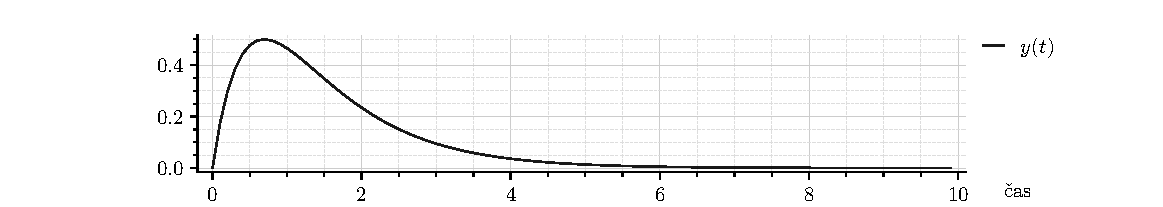
\includegraphics{ICH_SS2R_v1_p1.pdf}
        }

        \figcaption{Graf funkcie \eqref{fun_ICH_SS2R_v1}}
        \label{ICH_SS2R_v1_p1}
    }%vbox

\end{center}

Overme v MATLAB-e pomocou \lstinline|Symbolic Math Toolbox| a pomocou \lstinline|Control System Toolbox|:

% python .\jupynotex.py ..\MRS07_ICH2R_ML.ipynb '1-2' '70'

\input{../../PY/jupynotex/tex/MRS07_ICH2R_MLipynb_1-2.tex}


\subparagraph{Dva rovnaké reálne póly (jeden dvojnásobný pól).}

Zvoľme prípad, keď sú dva nezávislé reálne póly, teda napr. $p_1 = -1$ a $p_2 = -1$. Parameter $b_0$ zvoľme tak, že statické zosilnenie systému bude jednotkové, teda $b_0 = a_0$. 

Polynóm $A(s)$ je teda $A(s) = \left( s + 1 \right) \left( s + 1 \right) = s^2 + 2s + 1$ a~parameter $b_0 = 1$. Obraz výstupnej veličiny pri Dirackovom impulze na vstupe teda je
\begin{align}
    Y(s) = \frac{1}{s^2 + 2s + 1} = \frac{1}{(s + 1)(s + 1)} = \frac{1}{\left(s+1\right)^2}
\end{align}
Originál potom je
\begin{align} \label{fun_ICH_SS2R_v2}
    y(t) = te^{-t}  
\end{align}
\begin{center}

    \vbox{%
        \makebox[\textwidth][c]{%
        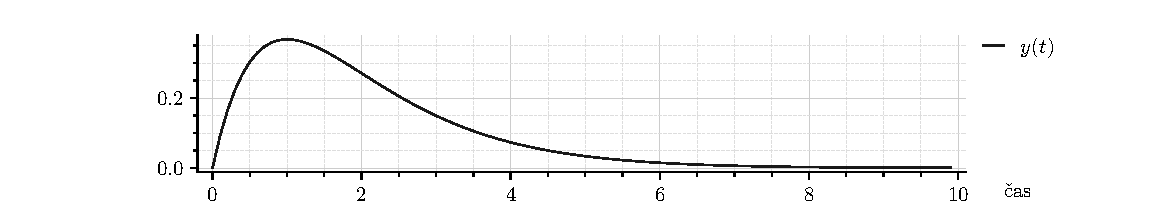
\includegraphics{ICH_SS2R_v2_p1.pdf}
        }

        \figcaption{Graf funkcie \eqref{fun_ICH_SS2R_v2}}
        \label{ICH_SS2R_v2_p1}
    }%vbox

\end{center}





\subparagraph{Dva komplexne združené póly.}

Ak by sme chceli póly systému, ktoré sú navzájom komplexne združenými číslami, potom je v prípade systému druhého rádu výhodné uvažovať charakteristický polynóm v tvare
\begin{align}
    A(s) = s^2 + 2 \beta \omega_0 s + \omega_0^2
\end{align}
kde $\beta$ a $\omega_0$ sú parametre, pričom $\beta$ sa nazýva koeficient tlmenia a $\omega_0$ sa nazýva vlastná frekvencia systému. Uvedené označovanie a forma polynómu $A(s)$ vyplývajú z konvencií pri opise oscilácií ako dynamického deja (diferenciálne rovnice tlmených oscilátorov). Ak je parameter $\beta < 1$, potom korene $A(s)$ sú komplexne združené čísla. Ak je parameter $\beta \geq 1$, potom korene $A(s)$ sú reálne.

Zvoľme $\beta = 0,5$ a $\omega_0 = 3$. Polynóm $A(s)$ je teda $A(s) = s^2 + 3s + 9 = \left( s + \frac{3}{2} + \frac{3}{2} \sqrt{3} j \right) \left( s + \frac{3}{2} - \frac{3}{2} \sqrt{3} j \right) $. Parameter $b_0$ zvoľme tak, že statické zosilnenie systému bude jednotkové, teda $b_0 = 9$. Obraz výstupnej veličiny pri Dirackovom impulze na vstupe teda je
\begin{align}
    \begin{aligned}
        Y(s) &= \frac{9}{s^2 + 3s + 9} \\
        &= \frac{9}{\left( s + \frac{3}{2} + \frac{3}{2} \sqrt{3} j \right) \left( s + \frac{3}{2} - \frac{3}{2} \sqrt{3} j \right)} \\
        &= \frac{A}{s + \frac{3}{2} + \frac{3}{2} \sqrt{3} j} + \frac{B}{s + \frac{3}{2} - \frac{3}{2} \sqrt{3} j}
    \end{aligned}
\end{align}
kde $A$ a $B$ sú konštanty, ktoré je potrebné nájsť. Platí
\begin{align}
    9 = A \left( s + \frac{3}{2} - \frac{3}{2} \sqrt{3} j \right) + B \left( s + \frac{3}{2} + \frac{3}{2} \sqrt{3} j \right)
\end{align}
Pre $s = - \frac{3}{2} - \frac{3}{2} \sqrt{3} j$ potom
\begin{align}
    \begin{aligned}
        9 &= A \left( - \frac{3}{2} - \frac{3}{2} \sqrt{3} j + \frac{3}{2} - \frac{3}{2} \sqrt{3} j \right) \\
        &= A \left( - 3 \sqrt{3} j   \right) 
    \end{aligned} 
\end{align}
\begin{align}    
        A &= \frac{9}{- 3 \sqrt{3} j} = \frac{3}{-  \sqrt{3} j} \cdot \frac{\sqrt{3} j}{\sqrt{3} j} = \frac{3 \sqrt{3} j}{3} = \sqrt{3} j
\end{align}
Pre $s = - \frac{3}{2} + \frac{3}{2} \sqrt{3} j$ potom
\begin{align}
    \begin{aligned}
        9 &= B \left( - \frac{3}{2} + \frac{3}{2} \sqrt{3} j + \frac{3}{2} + \frac{3}{2} \sqrt{3} j \right) \\
        &= B \left(  3 \sqrt{3} j   \right) 
    \end{aligned} 
\end{align}
\begin{align}    
    B &= \frac{9}{ 3 \sqrt{3} j} = \frac{3}{  \sqrt{3} j} \cdot \frac{-\sqrt{3} j}{-\sqrt{3} j} = \frac{-3 \sqrt{3} j}{3} = -\sqrt{3} j
\end{align}
Obraz výstupnej veličiny teda je
\begin{align}
        Y(s) &= \frac{\sqrt{3} j}{s + \frac{3}{2} + \frac{3}{2} \sqrt{3} j} - \frac{\sqrt{3} j}{s + \frac{3}{2} - \frac{3}{2} \sqrt{3} j}
\end{align}
Originál potom je
\begin{align} %
    \begin{aligned}
        y(t) &= \sqrt{3} j e^{- \frac{3}{2} \left(1 + \sqrt{3}j\right) t} - \sqrt{3} j e^{- \frac{3}{2} \left(1 - \sqrt{3}j\right) t} \\
        &= \sqrt{3} j \left( 
            e^{-\frac{3}{2}t}   
            e^{-\frac{3}{2}\sqrt{3}jt}
            -
            e^{-\frac{3}{2}t}   
            e^{\frac{3}{2}\sqrt{3}jt}
            \right)
            \\
        &= \sqrt{3} j e^{-\frac{3}{2}t}    \left(   
            e^{-\frac{3}{2}\sqrt{3}jt}
            -
            e^{\frac{3}{2}\sqrt{3}jt}
        \right)  
    \end{aligned}
\end{align}
Platí Eulerova identita $e^{j x} = \cos x + j \sin x$, teda 
\begin{subequations}
\begin{align} %
        y(t) 
        &= \sqrt{3} j e^{-\frac{3}{2}t}    \left(   
            \cos \left( -\frac{3}{2}\sqrt{3}t \right) 
            + j \sin \left( -\frac{3}{2}\sqrt{3}t \right)
            -
            \cos \left( \frac{3}{2}\sqrt{3}t \right)
            - j \sin \left( \frac{3}{2}\sqrt{3}t \right)
        \right) \\  
        y(t) 
        &= \sqrt{3} j e^{-\frac{3}{2}t}    \left(   
            + j \sin \left( -\frac{3}{2}\sqrt{3}t \right)
            - j \sin \left( \frac{3}{2}\sqrt{3}t \right)
        \right)  \\
        y(t) 
        &= \sqrt{3} j e^{-\frac{3}{2}t}  j  \left(   
            + \sin \left( -\frac{3}{2}\sqrt{3}t \right)
            - \sin \left( \frac{3}{2}\sqrt{3}t \right)
        \right) \\
        y(t) 
        &= - \sqrt{3} e^{-\frac{3}{2}t}   \left(   
            + \sin \left( -\frac{3}{2}\sqrt{3}t \right)
            - \sin \left( \frac{3}{2}\sqrt{3}t \right)
        \right)
\end{align}
\end{subequations}
Tiež platí $ \sin(-x) = - \sin(x)$ a teda
\begin{subequations}
\begin{align}
    y(t) &= - \sqrt{3} e^{-\frac{3}{2}t}  
    \left(   
        - 2 \sin \left( \frac{3}{2}\sqrt{3}t \right)
    \right) \\
    y(t) &= 2 \sqrt{3} e^{-\frac{3}{2}t}  \sin \left( \frac{3}{2}\sqrt{3}t \right) \label{fun_ICH_SS2R_v3}
\end{align}
\end{subequations}
\begin{center}

    \vbox{%
        \makebox[\textwidth][c]{%
        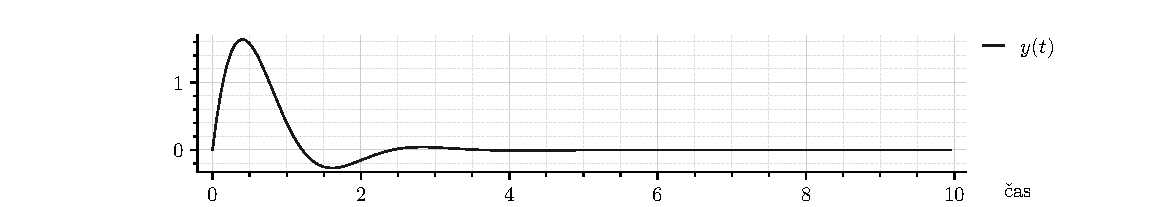
\includegraphics{ICH_SS2R_v3_p1.pdf}
        }

        \figcaption{Graf funkcie \eqref{fun_ICH_SS2R_v3}}
        \label{ICH_SS2R_v3_p1}
    }%vbox

\end{center}






\paragraph{ICH SS2R, prípad $B(s) = b_1 s + b_0$ alebo  $B(s) = b_1 s $}

Je zrejmé, že v prípade ak polynóm $B(s)$ je v tvare $B(s) = b_1 s + b_0$ alebo $B(s) = b_1 s$ má to vplyv na dynamiku systému.

Napríklad, pre polynóm $A(s)$ uvažujme situáciu rovnakú ako na obr.~\ref{ICH_SS2R_v1_p1}, teda póly systému sú $p_1 = -1$ a $p_2 = -2$, teda $A(s) = s^2 + 3s + 2$. Polynóm $B(s)$ zvoľme $B(s) = 3 s + 2$. V tomto prípade je nula systému, označme ju $z_1$, v bode $z_1 = -\frac{2}{3}$ a~teda táto nula sa nezhoduje so žiadnym pólom.

Obraz výstupnej veličiny pri Dirackovom impulze na vstupe je
\begin{align}
    Y(s) = \frac{3s + 2}{s^2 + 3s + 2} = \frac{3s + 2}{(s + 1)(s + 2)} = \frac{-1}{s + 1} + \frac{4}{s + 2}
\end{align}
Originál potom je
\begin{align} \label{fun_ICH_SS2R_v4}
    y(t) = -e^{-t} + 4e^{-2t}
\end{align}
\begin{center}

    \vbox{%
        \makebox[\textwidth][c]{%
        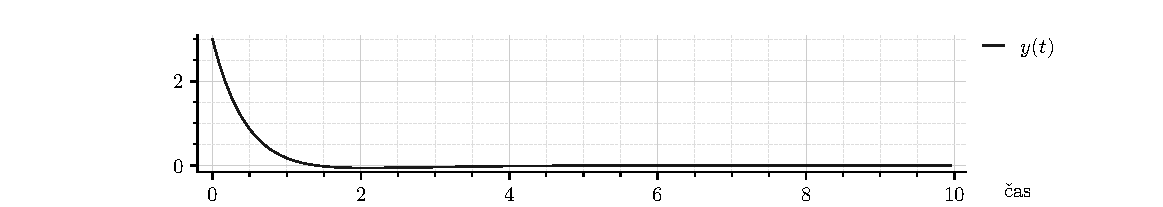
\includegraphics{ICH_SS2R_v4_p1.pdf}
        }

        \figcaption{Graf funkcie \eqref{fun_ICH_SS2R_v4}}
        \label{ICH_SS2R_v4_p1}
    }%vbox

\end{center}


Ak by sa nula zhodovala s pólom, teda napr bola by to $z_1 = -1$, potom by sme mali $G(s) =  \frac{s + 1}{s^2 + 3 s + 2}$, čo je možné zapísať aj ako $G(s) =  \frac{(s + 1)}{(s+1)(s+2)} =  \frac{1}{(s+2)}$, čo je systém prvého rádu.

Pre úplnosť uvažujme tu aj prípad keď $B(s) = b_1 s$. Zvoľme napríklad $b_1 = 3$. Zachovávame $A(s) = s^2 + 3 s + 2$. Všimnime si, že teraz máme $b_0 = 0$. To znamená, že zosilnenie systému, teda hodnota $b_0/a_0$ bude v tomto prípade nulové.

Obraz výstupnej veličiny pri Dirackovom impulze na vstupe je
\begin{align}
    Y(s) = \frac{3s}{s^2 + 3s + 2} = \frac{3s}{(s + 1)(s + 2)} = \frac{-3}{s + 1} + \frac{6}{s + 2}
\end{align}
Originál potom je
\begin{align} \label{fun_ICH_SS2R_v5}
    y(t) = -3e^{-t} + 6e^{-2t}
\end{align}
\begin{center}

    \vbox{%
        \makebox[\textwidth][c]{%
        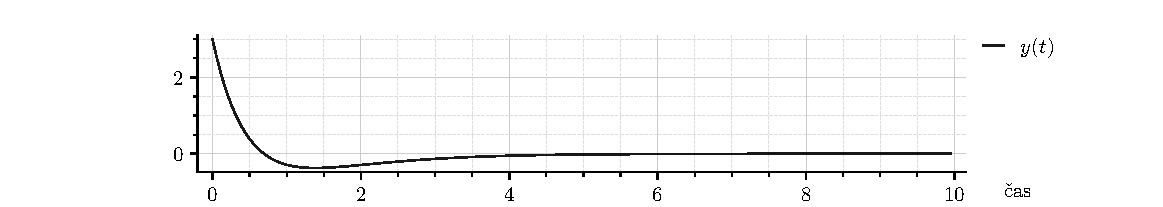
\includegraphics{ICH_SS2R_v5_p1.pdf}
        }

        \figcaption{Graf funkcie \eqref{fun_ICH_SS2R_v5}}
        \label{ICH_SS2R_v5_p1}
    }%vbox

\end{center}

Poznámka: póly systému sme tu zvolili čisto reálne (bez imaginárnej časti) a nie komplexne združené. Je zrejmé, že vplyv nuly na dynamiku systému má charakter kmitania a komplexne združené póly by túto skutočnosť v tejto ukážke zakryli, pretože sami vedú na kmitavú odpoveď systému.






\paragraph{ICH AS2R}

Ak je jeden z pólov systému nulový, hovoríme, že systém je astatický („obsahuje astatizmus“). Ak práve jeden pól je nulový, hovoríme o astatizme prvého rádu. Zvoľme tu $B(s) = 1$ a póly $p_1 = -1$ a $p_2 = 0$. Teda $A(s) = s^2 + s$.

Obraz výstupnej veličiny pri Dirackovom impulze na vstupe je
\begin{align}
    Y(s) = \frac{1}{s^2 + s} = \frac{1}{s(s + 1)} = \frac{1}{s} - \frac{1}{s + 1}
\end{align}
Originál potom je
\begin{align} \label{fun_ICH_AS2R_v1}
    y(t) = 1 - e^{-t}   
\end{align}
\begin{center}

    \vbox{%
        \makebox[\textwidth][c]{%
        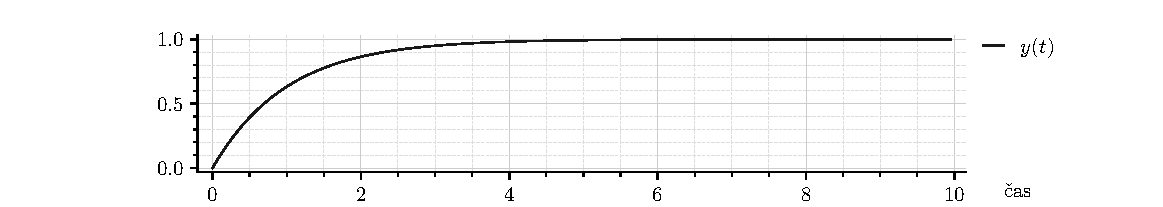
\includegraphics{ICH_AS2R_v1_p1.pdf}
        }

        \figcaption{Graf funkcie \eqref{fun_ICH_AS2R_v1}}
        \label{ICH_AS2R_v1_p1}
    }%vbox

\end{center}




Prípadne by sme mohli mať póly $p_1 = 0$ a $p_2 = 0$. Teda $A(s) = s^2$. Obraz výstupnej veličiny pri Dirackovom impulze na vstupe je
\begin{align}
    Y(s) = \frac{1}{s^2} 
\end{align}
Originál potom je
\begin{align} \label{fun_ICH_AS2R_v2}
    y(t) = t
\end{align}
\begin{center}

    \vbox{%
        \makebox[\textwidth][c]{%
        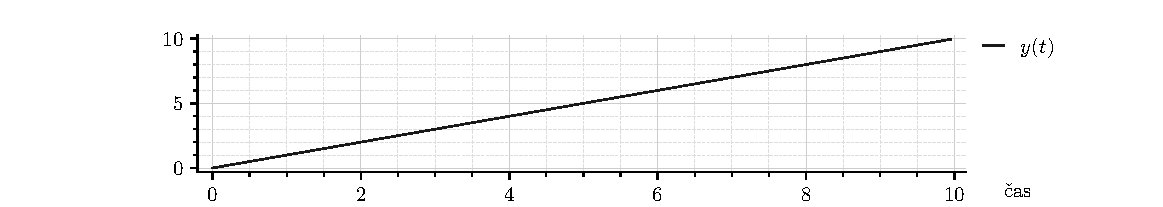
\includegraphics{ICH_AS2R_v2_p1.pdf}
        }

        \figcaption{Graf funkcie \eqref{fun_ICH_AS2R_v2}}
        \label{ICH_AS2R_v2_p1}
    }%vbox

\end{center}

Azda len pre zaujímavosť tu zvoľme $B(s) =  s + 1$, pritom ponechajme póly $p_1 = 0$ a~$p_2 = 0$, teda $A(s) = s^2$. Obraz výstupnej veličiny pri Dirackovom impulze na vstupe je
\begin{align}
    Y(s) = \frac{s + 1}{s^2} = \frac{1}{s} + \frac{1}{s^2}
\end{align}
Originál potom je
\begin{align} \label{fun_ICH_AS2R_v3}
    y(t) = 1 + t
\end{align}








\subsubsection{Prechodová charakteristika}


Prechodová charakteristika je odpoveď systému na jednotkový skok.

Keďže máme k dispozícii matematický opis systému, prechodovú charakteristiku môžeme	nájsť analyticky. Laplaceov obraz jednotkového skoku je $U(s) = \frac{1}{s}$.


\paragraph{PCH SS2R, prípad $B(s) = b_0$}

V prvom rade uvažujme prípad, keď dynamiku systému určujú len póly systému, teda prenosová funkcia je v tvare
\begin{align}
    G(s) =  \frac{b_0}{s^2 + a_1 s + a_0}
\end{align}


Polynóm $B(s) = b_0$ je nultého stupňa, teda systém nemá žiadne nuly. Označme póly systému $p_1$ a $p_2$. 

\subparagraph{Dva nezávislé reálne póly.}

Zvoľme prípad, keď sú dva nezávislé reálne póly, teda napr. $p_1 = -1$ a $p_2 = -2$. Parameter $b_0$ zvoľme tak, že statické zosilnenie systému bude jednotkové, teda $b_0 = a_0$. 

Polynóm $A(s)$ je teda $A(s) = \left( s + 1 \right) \left( s + 2 \right) = s^2 + 3s + 2$ a~parameter $b_0 = 2$. Obraz výstupnej veličiny pri jednotkovom skoku na vstupe je
\begin{align}
    Y(s) = \frac{2}{s^2 + 3s + 2} \frac{1}{s} = \frac{2}{(s + 1)(s + 2)} \frac{1}{s} = \frac{1}{s} - \frac{2}{s + 1} + \frac{1}{s + 2}
\end{align}
Originál potom je
\begin{align} \label{fun_PCH_SS2R_v1}
    y(t) = 1 - 2e^{-t} + e^{-2t}
\end{align}
\begin{center}

    \vbox{%
        \makebox[\textwidth][c]{%
        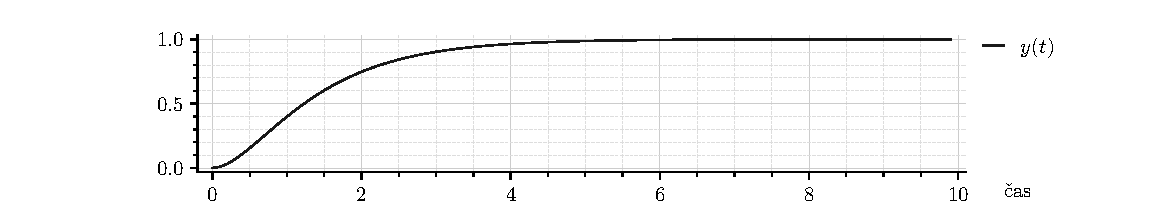
\includegraphics{PCH_SS2R_v1_p1.pdf}
        }

        \figcaption{Graf funkcie \eqref{fun_PCH_SS2R_v1}}
        \label{PCH_SS2R_v1_p1}
    }%vbox

\end{center}



\subparagraph{Dva rovnaké reálne póly (jeden dvojnásobný pól).}

Zvoľme prípad, keď sú dva nezávislé reálne póly, teda napr. $p_1 = -1$ a $p_2 = -1$. Parameter $b_0$ zvoľme tak, že statické zosilnenie systému bude jednotkové, teda $b_0 = a_0$. Polynóm $A(s)$ je teda $A(s) = \left( s + 1 \right) \left( s + 1 \right) = s^2 + 2s + 1$ a~parameter $b_0 = 1$. Obraz výstupnej veličiny pri jednotkovom skoku na vstupe je
\begin{align}
    Y(s) = \frac{1}{s^2 + 2s + 1} \frac{1}{s} = \frac{1}{(s + 1)(s + 1)} \frac{1}{s} = \frac{1}{(s + 1)^2} \frac{1}{s} =  \frac{-1}{(s + 1)^2} + \frac{-1}{s + 1} + \frac{1}{s}
\end{align}
Originál je
\begin{align} \label{fun_PCH_SS2R_v2}
    y(t) = -te^{-t} - e^{-t} + 1
\end{align}
\begin{center}

    \vbox{%
        \makebox[\textwidth][c]{%
        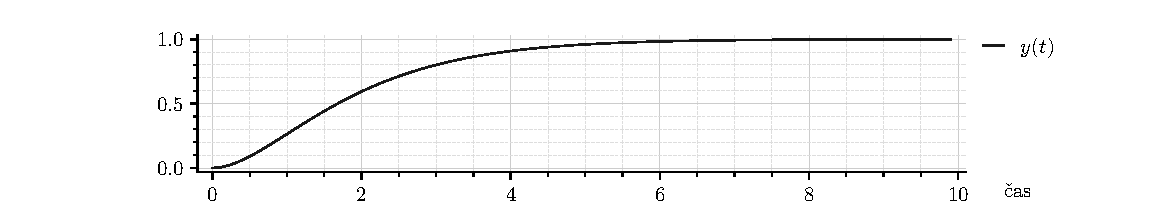
\includegraphics{PCH_SS2R_v2_p1.pdf}
        }

        \figcaption{Graf funkcie \eqref{fun_PCH_SS2R_v2}}
        \label{PCH_SS2R_v2_p1}
    }%vbox

\end{center}


\subparagraph{Dva komplexne združené póly.}

Ak by sme chceli póly systému, ktoré sú navzájom komplexne združenými číslami, potom je v prípade systému druhého rádu výhodné uvažovať charakteristický polynóm v tvare
\begin{align}
    A(s) = s^2 + 2 \beta \omega_0 s + \omega_0^2
\end{align}
kde $\beta$ a $\omega_0$ sú parametre, pričom $\beta$ sa nazýva koeficient tlmenia a $\omega_0$ sa nazýva vlastná frekvencia systému.

Zvoľme $\beta = 0,5$ a $\omega_0 = 3$. Polynóm $A(s)$ je teda $A(s) = s^2 + 3s + 9 = \left( s + \frac{3}{2} + \frac{3}{2} \sqrt{3} j \right) \left( s + \frac{3}{2} - \frac{3}{2} \sqrt{3} j \right) $. Parameter $b_0$ zvoľme tak, že statické zosilnenie systému bude jednotkové, teda $b_0 = 9$. Obraz výstupnej veličiny pri jednotkovom skoku na vstupe je
\begin{align}
    \begin{aligned}
        Y(s) &= \frac{9}{s^2 + 3s + 9} \frac{1}{s} 
    \end{aligned}
\end{align}
Originál je
\begin{align} \label{fun_PCH_SS2R_v3} 
    1-{{e}}^{-\frac{3\,t}{2}}\,\left(\cos\left(\frac{3\,\sqrt{3}\,t}{2}\right)+\frac{\sqrt{3}\,\sin\left(\frac{3\,\sqrt{3}\,t}{2}\right)}{3}\right)
\end{align}
čo bolo v tomto prípade určené s využitím \lstinline|Symbolic Math Toolbox| v~MATLAB-e ako ukazuje nasledujúci výpis kódu.
\begin{center}

    \vbox{%
        \makebox[\textwidth][c]{%
        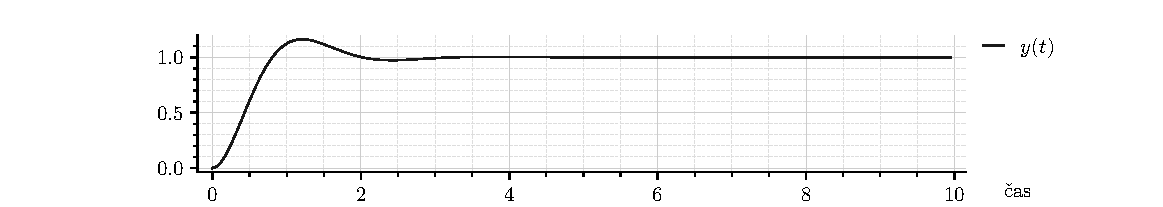
\includegraphics{PCH_SS2R_v3_p1.pdf}
        }

        \figcaption{Graf funkcie \eqref{fun_PCH_SS2R_v2}}
        \label{PCH_SS2R_v3_p1}
    }%vbox

\end{center}


% % python jupynotex.py ../MRS07_PCH2R_ML.ipynb '5' '70'
\input{../../PY/jupynotex/tex/MRS07_PCH2R_MLipynb_5.tex}


\paragraph{PCH SS2R, prípad $B(s) = b_1 s + b_0$ alebo  $B(s) = b_1 s $}

Je zrejmé, že v prípade ak polynóm $B(s)$ je v tvare $B(s) = b_1 s + b_0$ alebo $B(s) = b_1 s$ má to vplyv na dynamiku systému.

Napríklad, pre polynóm $A(s)$ uvažujme situáciu rovnakú ako na obr.~\ref{PCH_SS2R_v1_p1}, teda póly systému sú $p_1 = -1$ a $p_2 = -2$, teda $A(s) = s^2 + 3s + 2$. Polynóm $B(s)$ zvoľme $B(s) = 3 s + 2$. V tomto prípade je nula systému, označme ju $z_1$, v bode $z_1 = -\frac{2}{3}$ a~teda táto nula sa nezhoduje so žiadnym pólom. Obraz výstupnej veličiny pri jednotkovom skoku na vstupe je
\begin{align}
    Y(s) = \frac{3s + 2}{s^2 + 3s + 2} \frac{1}{s} = \frac{3s + 2}{(s + 1)(s + 2)} \frac{1}{s} = \frac{1}{s} + \frac{1}{s + 1} - \frac{2}{s + 2}
\end{align}
Originál je
\begin{align} \label{fun_PCH_SS2R_v4}
    y(t) = 1 + e^{-t} - 2e^{-2t}
\end{align}
\begin{center}

    \vbox{%
        \makebox[\textwidth][c]{%
        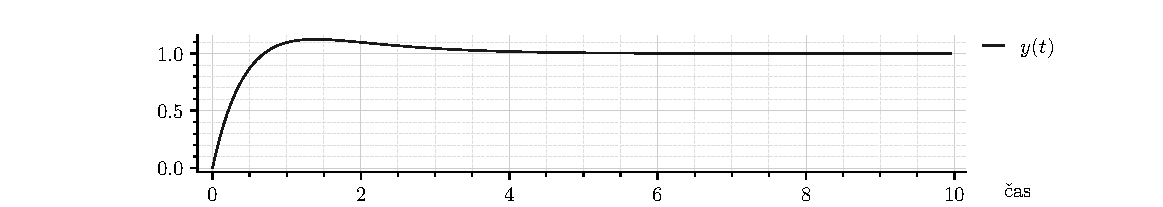
\includegraphics{PCH_SS2R_v4_p1.pdf}
        }

        \figcaption{Graf funkcie \eqref{fun_PCH_SS2R_v4}}
        \label{PCH_SS2R_v4_p1}
    }%vbox

\end{center}


Ak by sa nula zhodovala s pólom, teda napr bola by to $z_1 = -1$, potom by sme mali $G(s) =  \frac{s + 1}{s^2 + 3 s + 2}$, čo je možné zapísať aj ako $G(s) =  \frac{(s + 1)}{(s+1)(s+2)} =  \frac{1}{(s+2)}$, čo je systém prvého rádu.

Pre úplnosť uvažujme tu aj prípad keď $B(s) = b_1 s$. Zvoľme napríklad $b_1 = 3$. Zachovávame $A(s) = s^2 + 3 s + 2$. Všimnime si, že teraz máme $b_0 = 0$. To znamená, že zosilnenie systému, teda hodnota $b_0/a_0$ bude v tomto prípade nulové. Obraz výstupnej veličiny pri jednotkovom skoku na vstupe je
\begin{align}
    Y(s) = \frac{3s}{s^2 + 3s + 2} \frac{1}{s} = \frac{3s}{(s + 1)(s + 2)} \frac{1}{s} =  \frac{3}{s + 1} - \frac{3}{s + 2}
\end{align}
Originál je
\begin{align} \label{fun_PCH_SS2R_v5}
    y(t) = 3e^{-t} - 3e^{-2t}
\end{align}
\begin{center}

    \vbox{%
        \makebox[\textwidth][c]{%
        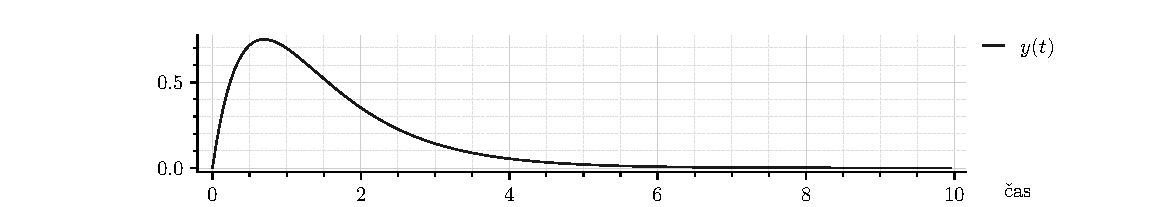
\includegraphics{PCH_SS2R_v5_p1.pdf}
        }

        \figcaption{Graf funkcie \eqref{fun_PCH_SS2R_v5}}
        \label{PCH_SS2R_v5_p1}
    }%vbox

\end{center}

Poznámka: póly systému sme tu zvolili čisto reálne (bez imaginárnej časti) a nie komplexne združené. Je zrejmé, že vplyv nuly na dynamiku systému má charakter kmitania a komplexne združené póly by túto skutočnosť v tejto ukážke zakryli, pretože sami vedú na kmitavú odpoveď systému.




\paragraph{PCH AS2R}

Ak je jeden z pólov systému nulový, hovoríme, že systém je astatický („obsahuje astatizmus“). Ak práve jeden pól je nulový, hovoríme o astatizme prvého rádu. Zvoľme tu $B(s) = 1$ a póly $p_1 = -1$ a $p_2 = 0$. Teda $A(s) = s^2 + s$. Obraz výstupnej veličiny pri jednotkovom skoku na vstupe je
\begin{align}
    Y(s) = \frac{1}{s^2 + s} \frac{1}{s} = \frac{1}{s(s + 1)} \frac{1}{s} = \frac{1}{s^2} - \frac{1}{s} + \frac{1}{s+1} 
\end{align}
Originál je
\begin{align} \label{fun_PCH_AS2R_v1}
    y(t) = t - 1 + e^{-t}
\end{align}
\begin{center}

    \vbox{%
        \makebox[\textwidth][c]{%
        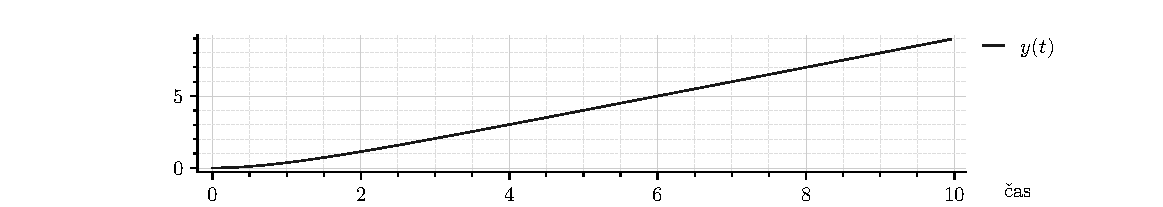
\includegraphics{PCH_AS2R_v1_p1.pdf}
        }

        \figcaption{Graf funkcie \eqref{fun_PCH_AS2R_v1}}
        \label{PCH_AS2R_v1_p1}
    }%vbox

\end{center}

Prípadne by sme mohli mať póly $p_1 = 0$ a $p_2 = 0$. Teda $A(s) = s^2$. Obraz výstupnej veličiny pri jednotkovom skoku na vstupe je
\begin{align}
    Y(s) = \frac{1}{s^2} \frac{1}{s} = \frac{1}{s^3}
\end{align}
Originál je
\begin{align} \label{fun_PCH_AS2R_v2}
    y(t) = \frac{t^2}{2}
\end{align}
\begin{center}

    \vbox{%
        \makebox[\textwidth][c]{%
        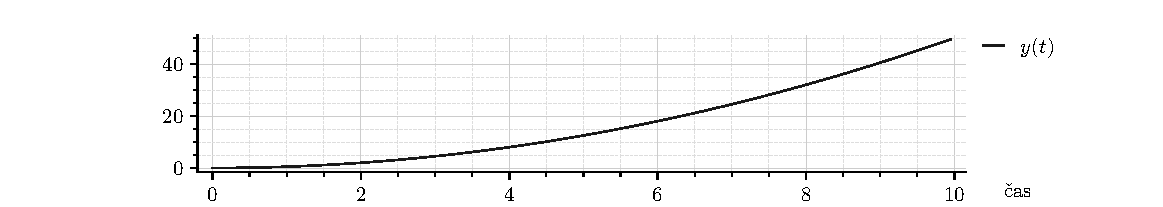
\includegraphics{PCH_AS2R_v2_p1.pdf}
        }

        \figcaption{Graf funkcie \eqref{fun_PCH_AS2R_v2}}
        \label{PCH_AS2R_v2_p1}
    }%vbox

\end{center}

Azda len pre zaujímavosť tu zvoľme $B(s) =  s + 1$, pritom ponechajme póly $p_1 = 0$ a~$p_2 = 0$, teda $A(s) = s^2$. Obraz výstupnej veličiny pri jednotkovom skoku na vstupe je
\begin{align}
    Y(s) = \frac{s + 1}{s^2} \frac{1}{s} = \frac{s + 1}{s^3} = \frac{1}{s^3} + \frac{1}{s^2}
\end{align}
Originál je
\begin{align} \label{fun_PCH_AS2R_v3}
    y(t) = \frac{t^2}{2} + t
\end{align}



























\printbibliography[title={Literatúra}]





\end{document}
